%chap04
\chap{BCS-BEC クロスオーバー領域における非磁性不純物効果}\label{chap:bcsl}

この章では、\ref{chap:formalism} 章で定式化した理論を用い、フェルミ原子気体の BCS-BEC クロスオーバー領域における非磁性不純物効果を数値計算により研究する。\ref{sec:bcsl:bsi} 節で、絶対零度の超流動秩序パラメータ $\del$ の不純物濃度 $\overline{c}$ 依存性、および不純物散乱長 $\bskfi$ 依存性を BCS-BEC クロスオーバー全域で明らかにする。またユニタリ極限において、1 粒子状態密度に対する不純物効果を議論する。\ref{sec:bcsl:bsi:iasvsibs} 節では、不純物散乱と原子間相互作用の競合現象を説明する。\ref{sec:bcsl:bsi:spectl} 節では超流動状態における 1 粒子スペクトルに対する不純物効果を考える。\ref{sec:bcsl:con} 節では、ユニタリ極限 $\askfi=0$ における超流動転移温度 $\tc$ に対する不純物効果を明らかにする。
åß
\s{絶対零度の超流動秩序パラメータに対する非磁性不純物効果}\label{sec:bcsl:bsi}

$T=0$ の超流動相を考える場合、パラメータとしては、原子間相互作用に対する $s$ 波散乱長 $\askfi$ [式 (\ref{eq:form:ham:askf})]、不純物散乱長 $\bskfi$ [式 (\ref{eq:form:ham:bskf})]、および不純物濃度 $\lc$ [式 (\ref{eq:form:ham:overlinec})] の 3 つである。現実のフェルミ原子気体では今のところ磁場によるフェッシュバッハ共鳴の制御を通じて変化させられる散乱長は $\askfi$ か $\bskfi$ のいずれか 1 つであるが、以下ではこれらを独立に変化させ、BCS-BEC クロスオーバー領域での非磁性不純物効果を調べる。

式 (\ref{eq:form:ham:himp}) の非磁性不純物散乱を表すハミルトニアンは、1 つの非磁性不純物が擬スピン $\spin=\uar$ と $\spin=\dar$ の両方と散乱する。したがって式 (\ref{eq:form:ham:overlinec}) の定義を用いる場合、不純物に束縛されるほど不純物散乱の効果が強い場合、$\lc=0.5$ の時に全てのフェルミ原子が不純物に束縛される状況が実現する。

\begin{figure}[t]
\centering
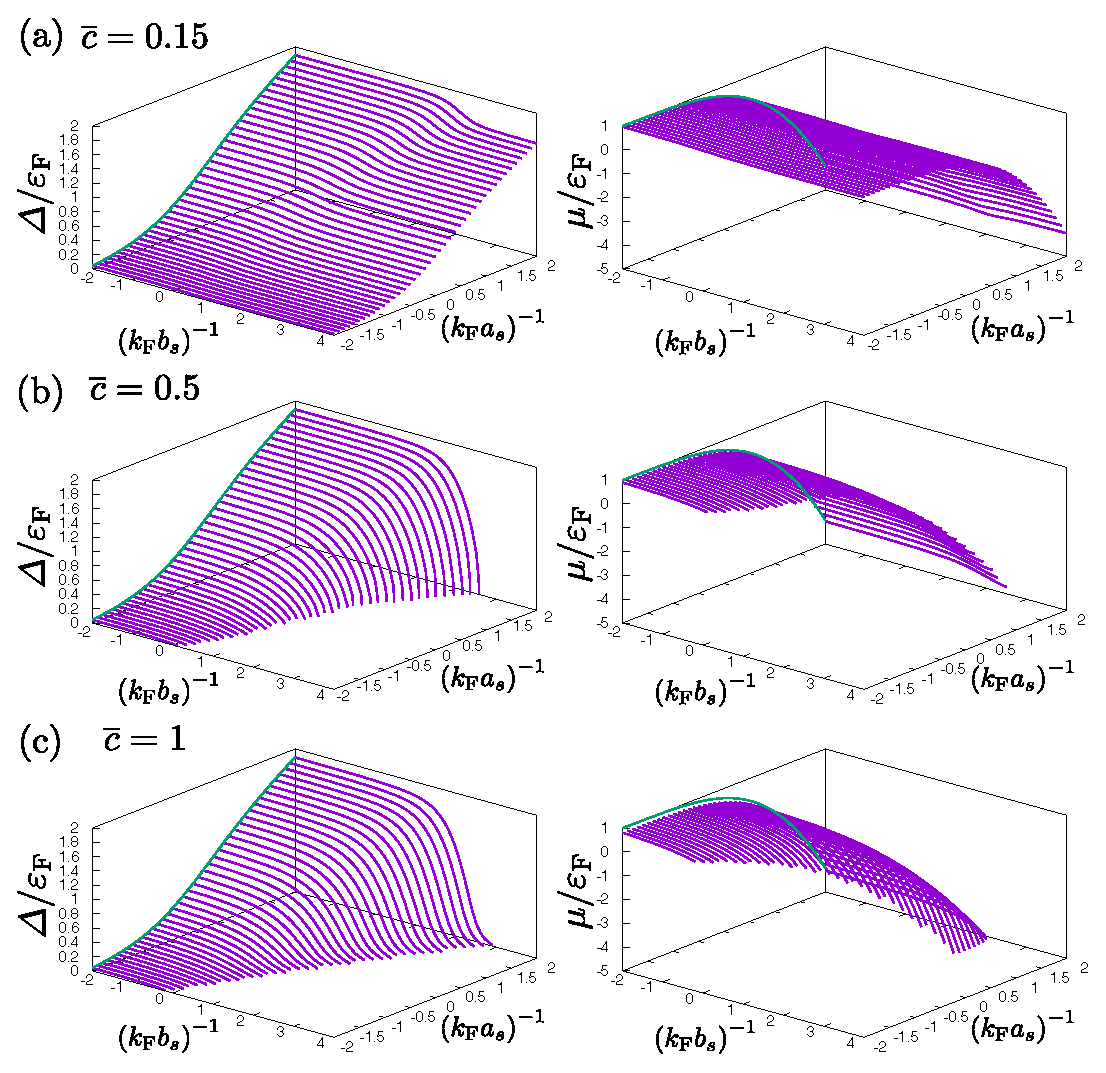
\includegraphics[width=130mm]{eps/sp-tc-cpt.eps}
\caption{$T=0$ の BCS-BEC クロスオーバー領域における超流動秩序パラメータ $\del$(左)と $\cpt$(右)。$\askfi$ は原子間相互作用強度、$\bskfi$ は不純物散乱強度を表す。各図の $\bskfi = -2$ における緑実線は付録 \ref{sec:append:pure:bcsl} で求めたクリーンな系における計算結果。}
\label{fig:bcsl:imp:cccc}
\end{figure}

ダイソン方程式 (\ref{eq:form:mnf:tomn}), (\ref{eq:form:mnf:tcptn}), (\ref{eq:form:mnf:nonmag})、ギャップ方程式 (\ref{eq:form:mnf:gapeq}), そして粒子数方程式 (\ref{eq:form:mnf:numeq}) を自己無撞着に解いて求めた $T=0$ での超流動秩序パラメータ $\del$、および化学ポテンシャル $\cpt$ を図 \ref{fig:bcsl:imp:cccc} に示す。いずれの場合も不純物散乱効果が弱い $\bskfi=-2$ では不純物を含まないクリーンな系での結果(緑実線:付録 \ref{sec:append:pure:bcsl} 参照)に近い。


\begin{figure}[t]
\centering
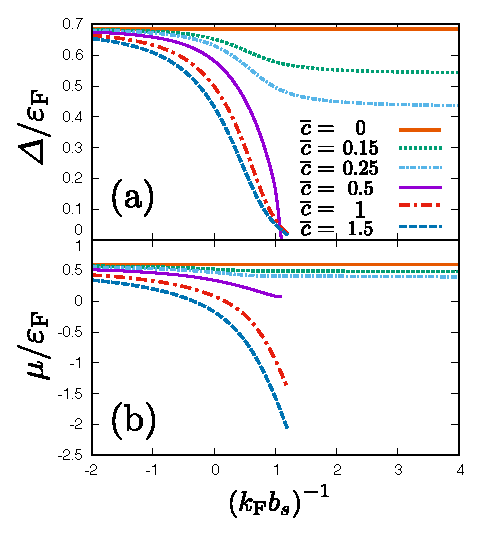
\includegraphics[width=90mm]{eps/bcsl-del-cpt-ias000.eps}
\caption{ユニタリ極限 $\left(\askfi=0\right)$ における (a) 超流動秩序変数 $\del$、 (b) 化学ポテンシャル $\cpt$、の不純物効果 $\lc = 0 $ の結果は不純物がない場合の結果。}
\label{fig:bcsl:imp:ias000}
\end{figure}


不純物濃度が低い $\lc=0.15$ の場合、図 \ref{fig:bcsl:imp:cccc} (a)に示すように、不純物散乱長 $\bskfi$ が強くなると、超流動秩序パラメータは小さくなるものの最終的に有限な一定値に漸近する。一方、不純物濃度が $\lc = 0.5$ の場合、不純物散乱強度を強くすると超流動秩序パラメータが消失する(図 \ref{fig:bcsl:imp:cccc} (b))。さらに不純物濃度 $\lc$ を大きくすると、$\lc=1$ では、図 \ref{fig:bcsl:imp:cccc} (c)、あるいは図 \ref{fig:bcsl:imp:ias000} (a) に示すように、$\bskfi\sim 1$ 付近から $\lc=0.5$ に比べると減少が緩やかになり、$\bskfi\ge1.1$ では $\lc=0.5$ の値より大きくなる。今の計算では十分低温であるが、計算の都合上有限温度($T=0.01 \eqf$)を考えているため $\lc > 0.5$ の $\bskfi \gtsim 1.1$ での $\del$ は求まっていないが、\ref{sec:bcsl:dos-imp} 節の図 \ref{fig:bcsl:imp:large-c-dos} で議論する不純物バンド内での超流動秩序の形成という結果と組み合わせることにより、小さいが有限な $\varDelta$ は残り続けると考えられる(つまり超流動相は維持される)。

\s{1 粒子状態密度に対する不純物効果}\label{sec:bcsl:dos-imp}



\begin{figure}[t]
\centering
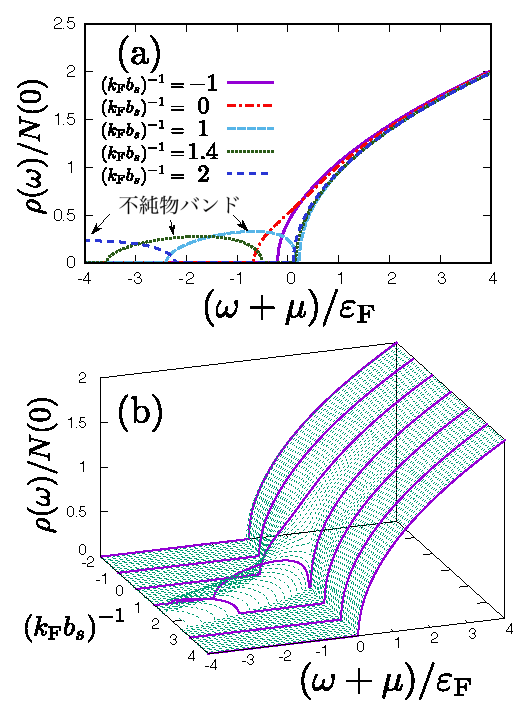
\includegraphics[width=80mm]{eps/normal-dos-c0500-2.eps}
\caption{自由フェルミ気体の状態密度に対する不純物散乱の効果(原子間引力相互作用は $U$ としている)。$\lc=0.5$。 (a) は典型的な散乱強度 $\bskfi$ に対する結果をプロットしてある。(b) は $-4 \le \bskfi \le 4$ での状態密度を表している。}
\label{fig:bcsl:imp:ndosc0500}
\end{figure}


通常の金属超伝導と異なり、アンダーソンの定理が成立せずに超流動秩序パラメータ $\del$ の大きさが不純物散乱強度 $\bskfi$ に依存することは不純物散乱の 1 粒子状態密度への影響の結果として理解できる。これを見るために図 \ref{fig:bcsl:imp:ias000} で $\del$ が $\bskfi \simeq 1.1$ で消失する $\lc=0.5$ の場合を考えると、「常流動相」における 1 粒子状態密度 $\rho(\omega)$ は図 \ref{fig:bcsl:imp:ndosc0500} のようになる($\rho(\omega)$ の計算方法は付録 \ref{sec:append:dosodosdoododosdosodosda} 参照)。一般に 2 体問題を考えると散乱長(今の場合は $\bs$)が負から正に変わると、束縛状態が形成されるようになるが、それを反映し、図 \ref{fig:bcsl:imp:ndosc0500} の状態密度は $\bskfi=0$ あたりからバンドの底に不純物散乱の影響が見えはじめ $\bskfi\geq 1$ では不純物バンドが現れることがわかる。この不純物バンドに収容できるフェルミ原子数は $\lc=0.5$ の場合、1 不純物当り擬スピン $\sigma=\uar, \dar$ の 2 個が束縛できることから全フェルミ原子数 $N$ に等しい。つまり下側の不純物バンドは“完全につまった”状態、つまり金属電子系との対応ではバンド絶縁体となる。このため、絶縁体が超伝導にならないのと同様、今の場合も $\bskfi$ から強くなり通常の“伝導バンド”の下に不純物バンドが形成され、そこに全てのフェルミ原子が(束縛状態という形で)収容され絶縁体になると超流動状態が消失するのである。

\begin{figure}[t]
\centering
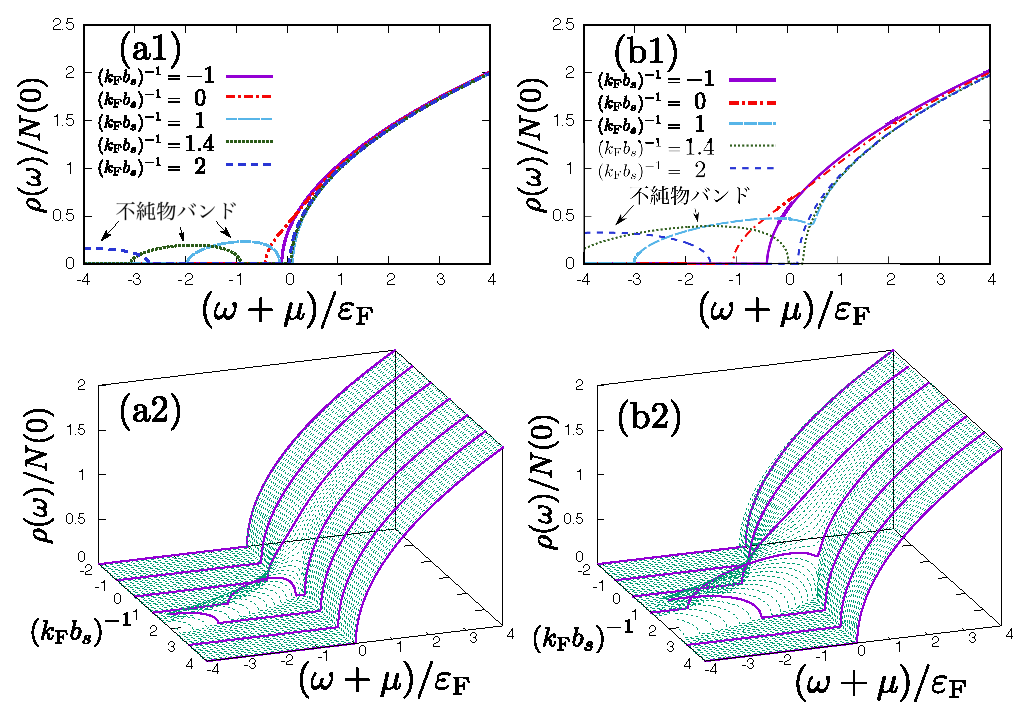
\includegraphics[width=130mm]{eps/normal-dos-c2-2.eps}
\caption{図 \ref{fig:bcsl:imp:ndosc0500} と同じであるが、濃度が (a1), (a2) $\lc=0.25$、(b1), (b2) $\lc=1$ の場合}
\label{fig:bcsl:imp:ndoscccc}
\end{figure}



上の議論で出て来た $\bskfi>0$ での不純物とフェルミ原子との束縛状態は 2 体問題であり、不純物濃度に関係なく現れる。実際、図 \ref{fig:bcsl:imp:ndoscccc} に示すように、$\lc=0.25$、$\lc=1$ でも $\bskfi\gtsim0$ になるとやはりバンドの底に不純物散乱の影響が見え始め、ついには不純物バンドが形成される。ただし、$\lc =0.5$ の場合と異なるのは、例えば $\lc=0.25$ の場合(図 \ref{fig:bcsl:imp:ndoscccc} (a1), (a2))、不純物バンドに収容できる原子は 1 不純物当たりの束縛原子数が 2 であることから $N/2$ であり、結果残りの $N/2$ のフェルミ原子は上の“伝導バンド”を占有、フェルミ面を形成する。したがって完全に占有された不純物バンド(=“絶縁”状態)を無視すると、系は $N/2$ 個のフェルミ原子からなる気体と考えられ、引力相互作用があればこれらの原子は不純物がない場合同様 $T=0$ で超流動状態になる。図 \ref{fig:bcsl:imp:ias000} (a) で $\lc<0.5$ の場合、$\bskfi>1$ でも $\del$ が有限に残るのはこのためである。また、この低不純物濃度で $\bskfi$ が大きくなると化学ポテンシャル $\cpt$ が低下、$\bskfi\gtsim1$ で一定値になるのも上記の議論から理解することができる。
\begin{figure}[t]
\centering
\subfigure[$\bskfi=-1$]{
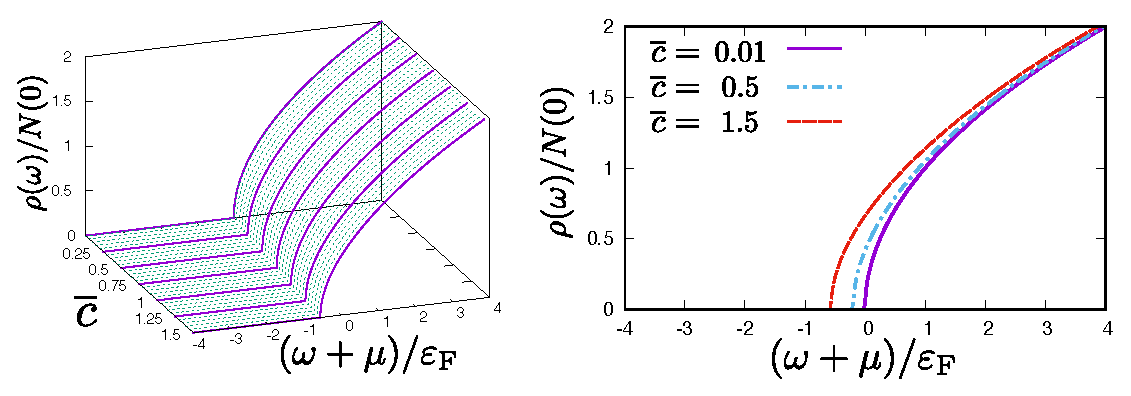
\includegraphics[width=120mm]{eps/ndos-ibs-1.eps}
}
\subfigure[$\bskfi=0$]{
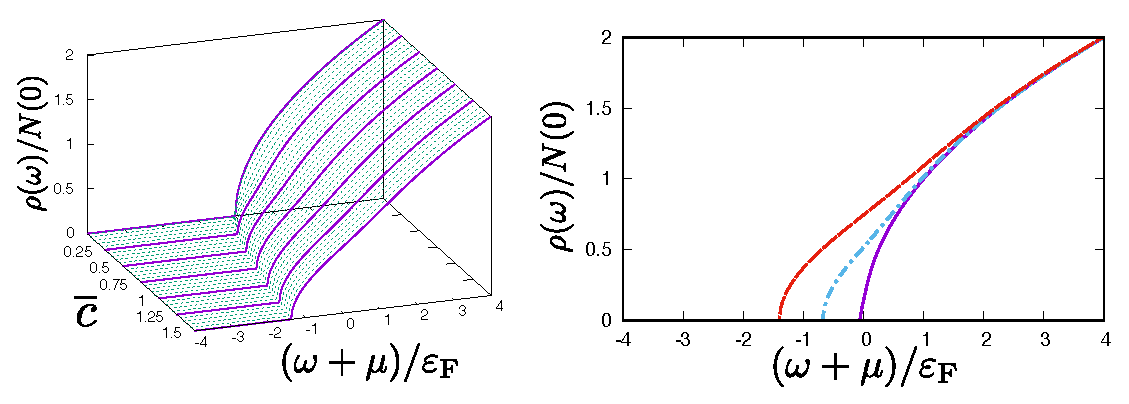
\includegraphics[width=120mm]{eps/ndos-ibs00.eps}
}
\subfigure[$\bskfi=1$]{
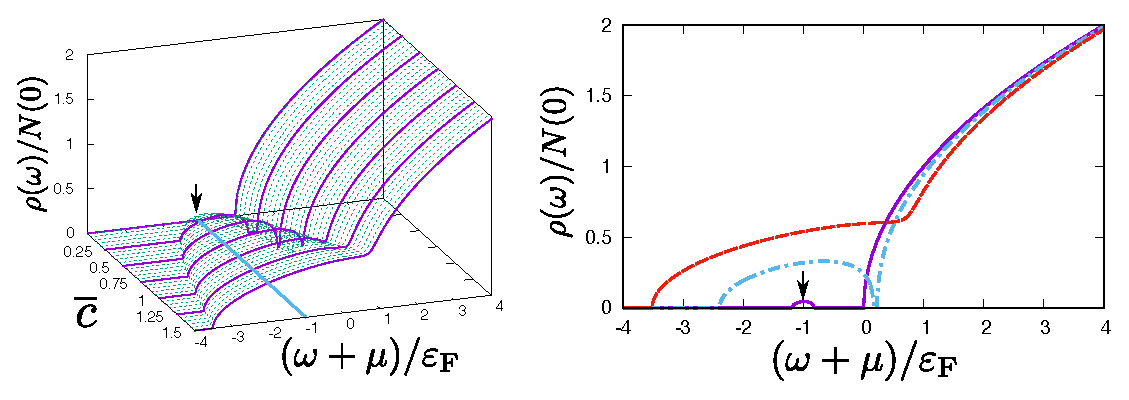
\includegraphics[width=120mm]{eps/ndos-ibs+1.eps}
}
\caption{自由フェルミ原子ガスの状態密度に対する不純物効果。(a) $\bskfi=-1$。(b) $\bskfi=0$。 (c) $\bskfi=1$。$\rho(\omega)$ は 1 粒子状態密度。いくつかの濃度に対する結果を右図に示す。(c) における矢印は不純物の束縛エネルギー(式 (\ref{eq:bcsl:bsi:eimpbind}))。}
\label{fig:bcsl:imp:ndosibs}
\end{figure}

一方、$\lc>0.5$ の場合、例えば $\lc=1$ では不純物バンドには $2N$ のフェルミ原子が占有可能であることから、$N$ 個のフェルミ原子ガスでは不純物バンドは部分的に収容される。結果、この不純物バンド内で超流動状態が生じることが期待される。今の計算では $T/T_{\text{F}} = 0.01$ の有限温度で計算しているため、$T=0$ での $\del$ がこの温度より小さい領域は、この温度効果が無視できず、図 \ref{fig:bcsl:imp:ias000} に示すように $\bskfi\gtsim 1$ での $\lc>0.5$ の結果は得られていないが、$T=0$ での計算を行えば非常に小さいながら有限な $\del$ がこの領域でも得られると考えられる。

2 体問題の範囲内で不純物束縛状態は $\bskfi>0$ で生じ、束縛エネルギー $E^{\imp}_{\text{bind}}$ は、
\beq
E^{\imp}_{\text{bind}} = - \frac{\eqf}{(\bskf)^2},\label{eq:bcsl:bsi:eimpbind}
\eeq
となる。実際、図 \ref{fig:bcsl:imp:ndosibs} に示すように、不純物バンドは $\bskfi>0$ の時、式 (\ref{eq:bcsl:bsi:eimpbind}) のエネルギーのまわりに拡がる形で現れる。その広がりのエネルギー幅は不純物濃度 $\lc$ が大きくなると不純物の束縛状態間の干渉が強くなる結果、大きくなり、ある程度濃度が高くなると上の“伝導バンド”と重なるようになる。この状態になると、その中にフェルミ準位を有するフェルミ原子ガスとなる。


\begin{figure}[t]
\centering
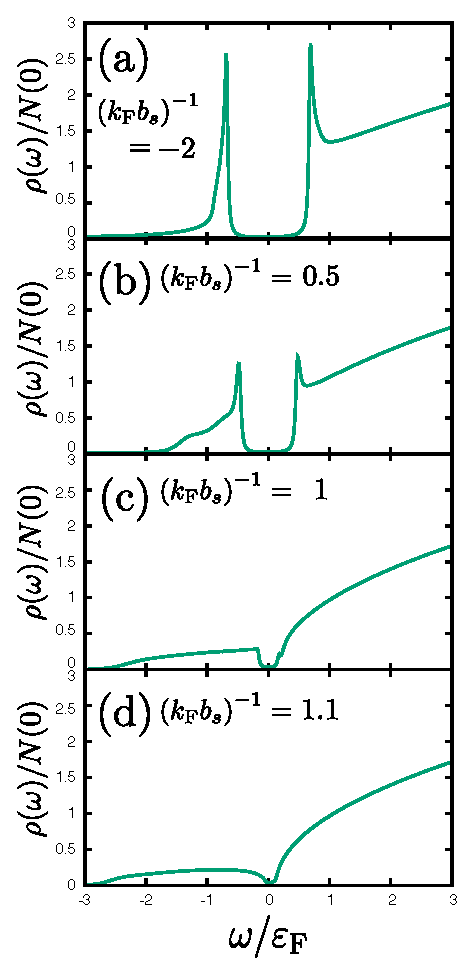
\includegraphics[width=60mm]{eps/bcsl-dos-c0500s.eps}
\caption{ユニタリー極限 $\askfi$=0、$T=0$ での超流動状態密度 $\rho(\omega)$。不純物濃度は $\lc=0.5$。}
\label{fig:bcsl:imp:bdosc0500ias000}
\end{figure}


\begin{figure}[t]
\centering
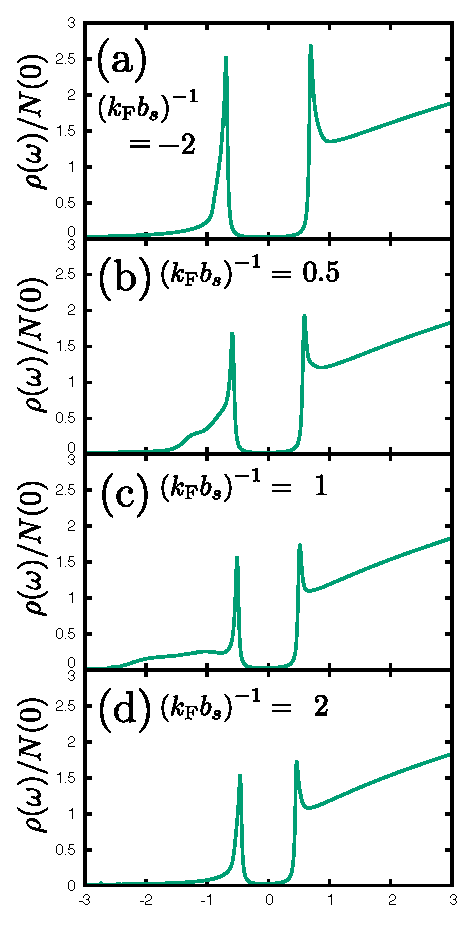
\includegraphics[width=60mm]{eps/bcsl-dos-c0250s.eps}
\caption{図 \ref{fig:bcsl:imp:bdosc0500ias000} と同じであるが、不純物濃度が $\lc=0.25$ の場合。}
\label{fig:bcsl:imp:bdosc0250ias000}
\end{figure}


図 \ref{fig:bcsl:imp:bdosc0500ias000} は、$\del$ が $\bskfi=1.1$ で $\del$ が消失する $\lc=0.5$ の場合のユニタリ極限における超伝導状態密度である。散乱効果が弱い $\bskfi = -2$ の場合はクリーンな系の超伝導状態密度とほとんど同じ結果が得られる。この状態密度は散乱強度が弱い $\bskfi=0.5$ まで大きくなると、自由フェルミ気体の状態密度の底が変形することを反映し、ギャップ構造も小さくなる。不純物バンドがちょうど分離する $\bskfi=1$ となると、自由粒子の状態密度と不純物バンドが近いため、両側の状態を利用して、超流動秩序を確保していることが見てとれる。このコヒーレンスピークは $\bskfi=1.1$ になると、不純物バンドとの間隔が大きくなることで完全に消え、超流動状態が消失する。


図 \ref{fig:bcsl:imp:bdosc0250ias000} は $\lc=0.25$ の場合のユニタリ極限における超伝導状態密度である。前述したように、この場合は $\bskfi>0$ でフェルミ原子の一部が不純物に束縛された後も $N/2$ 個のフェルミ原子が“伝導バンド”を占有するため超流動状態が保持される。これを反映し、状態密度に現れるギャップ構造も“伝導バンド”の原子数が減少するために小さくなるが $\lc=0.5$ の時(図 \ref{fig:bcsl:imp:bdosc0500ias000})とは異なり $\bskfi > 1.1 $ でも残り続ける。


\begin{figure}[t]
\centering
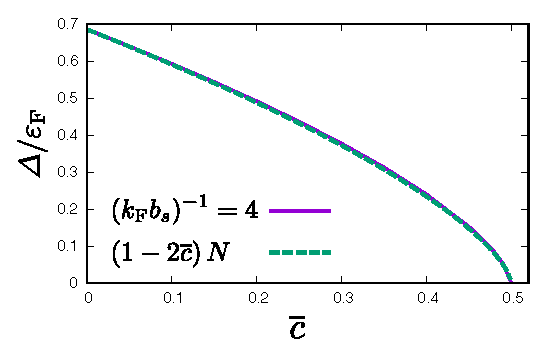
\includegraphics[width=90mm]{eps/bcsl-small-c.eps}
\caption{ユニタリー極限 $\askfi$=0、不純物散乱長 $\bskfi=4$ での超流動秩序パラメータ $\del$ の不純物濃度 $\overline{c}$ 依存性。実線は不純物 BCS-Leggett 理論の結果。破線は 式 (\ref{eq:bcsl:bsi:condelimp})。}
\label{fig:bcsl:imp:bcsl-ias000-condep}
\end{figure}


$\lc < 0.5$ では $\bskfi \gg 1$ で $\lc \times 2 N$ のフェルミ原子が不純物に束縛されるため $N\left(1-2\lc\right)$ が“伝導バンド”に残るが、実際、この評価でこの領域で計算された励起ギャップ(あるいは超流動秩序パラメータ $\del$)の値を説明できるか調べる。$\overline{N}=(1-2\lc)N$ 個のフェルミ原子ガスを考えると、その時のフェルミ波数 $\overline{k}_{\text{F}}$ は、
\beq
\overline{k}_{\text{F}} = \left[ 3 \pi^2 \left(1-2 \lc \right) N \right]^{\frac{1}{3}},
\eeq
となる。よってこの時のフェルミエネルギー $\overline{\ken}_{\text{F}}$ は、
\beq
\overline{\ken}_{\text{F}} &=  \frac{\overline{k}_{\text{F}}^2}{2m} \notag\\
&= \left(1-2 \lc\right)^{\frac{2}{3}} \eqf,
\eeq
となる。この“$\left(1-2 \lc\right)N$”粒子系の超流動秩序パラメータ $\overline{\del}$ は、
\beq
\frac{\overline{\varDelta}}{\overline{\ken}_{\text{F}}} = \frac{\del}{\eqf},
\eeq
の関係を満たすので、
\beq
\overline{\del} = \left(1-2\lc\right)^{\frac{2}{3}} \del, \label{eq:bcsl:bsi:condelimp}
\eeq
となることが期待される。実際、$\bskfi=4$ の場合に、計算される超流動秩序パラメータ $\del$ の不純物濃度 $\lc$ 依存性と式 (\ref{eq:bcsl:bsi:condelimp}) を比べると図 \ref{fig:bcsl:imp:bcsl-ias000-condep} に示すように両者はよく一致する。



\begin{figure}[t]
\centering
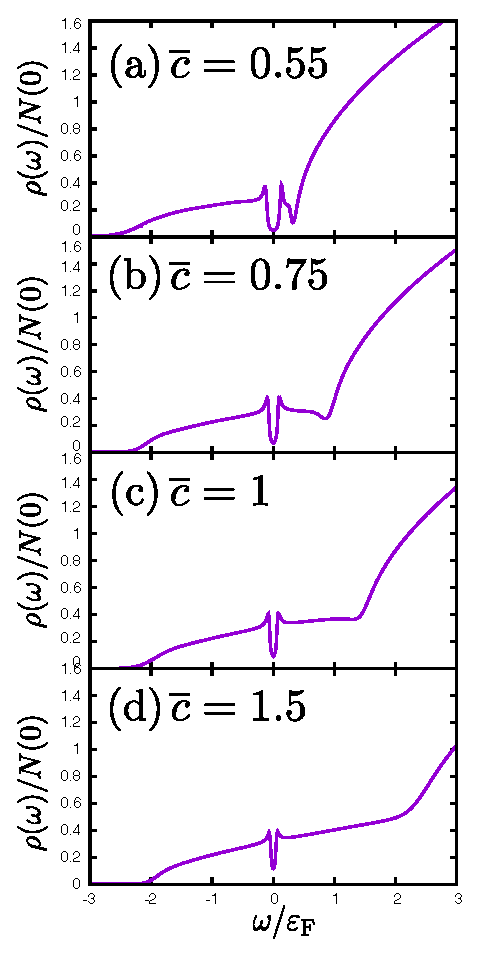
\includegraphics[width=60mm]{eps/bcsl-large-c.eps}
\caption{ユニタリー極限 $\askfi$=0、$T=0$ での超流動状態密度 $\rho(\omega)$。不純物散乱強度は $\bskfi=1$ にとってある。}
\label{fig:bcsl:imp:large-c-dos}
\end{figure}

図 \ref{fig:bcsl:imp:large-c-dos} はユニタリ極限における $\bskfi=1$ での超流動状態密度の不純物濃度依存性である。 $\lc\ge0.55$ の結果において、状態密度を $\omega/\eqf = 4$ から低エネルギー側へ見ていくと、窪み構造が見られる(例えば $\lc=0.75$ では、$\omega/\eqf\simeq 0.9$ (図 \ref{fig:bcsl:imp:large-c-dos} (c)))。これは上側の“伝導バンド”と下側の“不純物バンド”の境目である。このことに留意すると、$\lc>0.5$ の時超流動ギャップは“不純物バンド”内に形成されていることが見てとれる。これは $\lc > 0.5$ では不純物バンドの収容する粒子が $N$ より大きいため、“フェルミ準位”が不純物バンド内に存在することに因るものである。



\s{原子間引力相互作用と不純物散乱の競合}\label{sec:bcsl:bsi:iasvsibs}

式 (\ref{eq:bcsl:bsi:eimpbind}) に記したように $\bskfi>0$ の時、不純物周辺に形成される束縛状態の束縛エネルギーは $E^{\imp}_{\text{bind}} = -\eqf/(\bskf)^2$ である。一方で、付録 \ref{sec:append:pure} に示したように、原子間引力相互作用も $\askfi>0$ では 2 体レベルでの束縛状態の形成が可能となり、その“分子ボソン”の結合エネルギーは、
\beq
E_{\text{bind}}^{\as} = - \frac{\eqf}{(\askf)^2},\label{eq:bcsl:bsi:ebindas}
\eeq
となる。前者の束縛状態と異なるのは後者は空間的に“固定”されていない分子状態なので、このような分子で構成されるボース気体は BEC を起こす。結果として、この 2 種類の競合で超流動状態に影響を与える。

\begin{figure}[t]
\centering
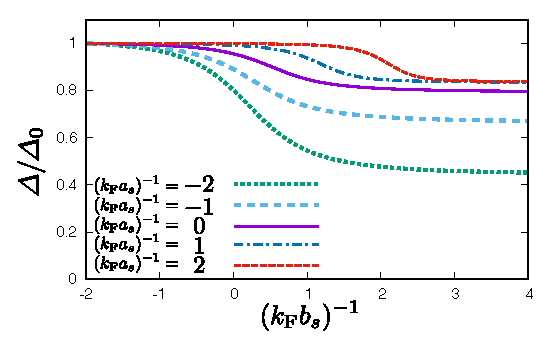
\includegraphics[width=100mm]{eps/bcsl-ias-ibs.eps}
\caption{超流動秩序パラメータ $\varDelta$ の不純物散乱長依存性。不純物濃度は $\lc=0.15$。$\del_0$ は各相互作用強度において不純物がない場合の超流動秩序パラメータ。}
\label{fig:bcsl:imp:ibs-vs-ias}
\end{figure}

図 \ref{fig:bcsl:imp:ibs-vs-ias} は、不純物がない場合の値で規格化した不純物濃度 $\lc=0.15$ の超流動秩序パラメータ $\del$ の不純物散乱長 $\bskfi$ 依存性である。引力相互作用が 2 体束縛状態を作らない $\askfi\le 0$ では、$\bskfi=0$ 付近から超流動秩序パラメータ $\del$ が減少していることが分かる。これは $\bskfi=0$ で不純物が状態密度の底に影響を与え始め、不純物バンドの形成へと向かうためである。一方 $\askfi > 0$ では、式 (\ref{eq:bcsl:bsi:ebindas}) で与えられる結合エネルギーを有する分子ボソンが形成されるため、それを上回る結合エネルギーを有する不純物束縛状態が現れはじめる状況($|E_{\text{bind}}^{\bs}| > |E_{\text{bind}}^{\as}|$) すなわち $\bskfi>\askfi$ となる領域にさしかかったあたりから超流動秩序パラメータが減少しはじめる。この時、相互作用による分子ボソンが一部解離し、かわって不純物束縛状態が形成される。


\begin{figure}[t]
\centering
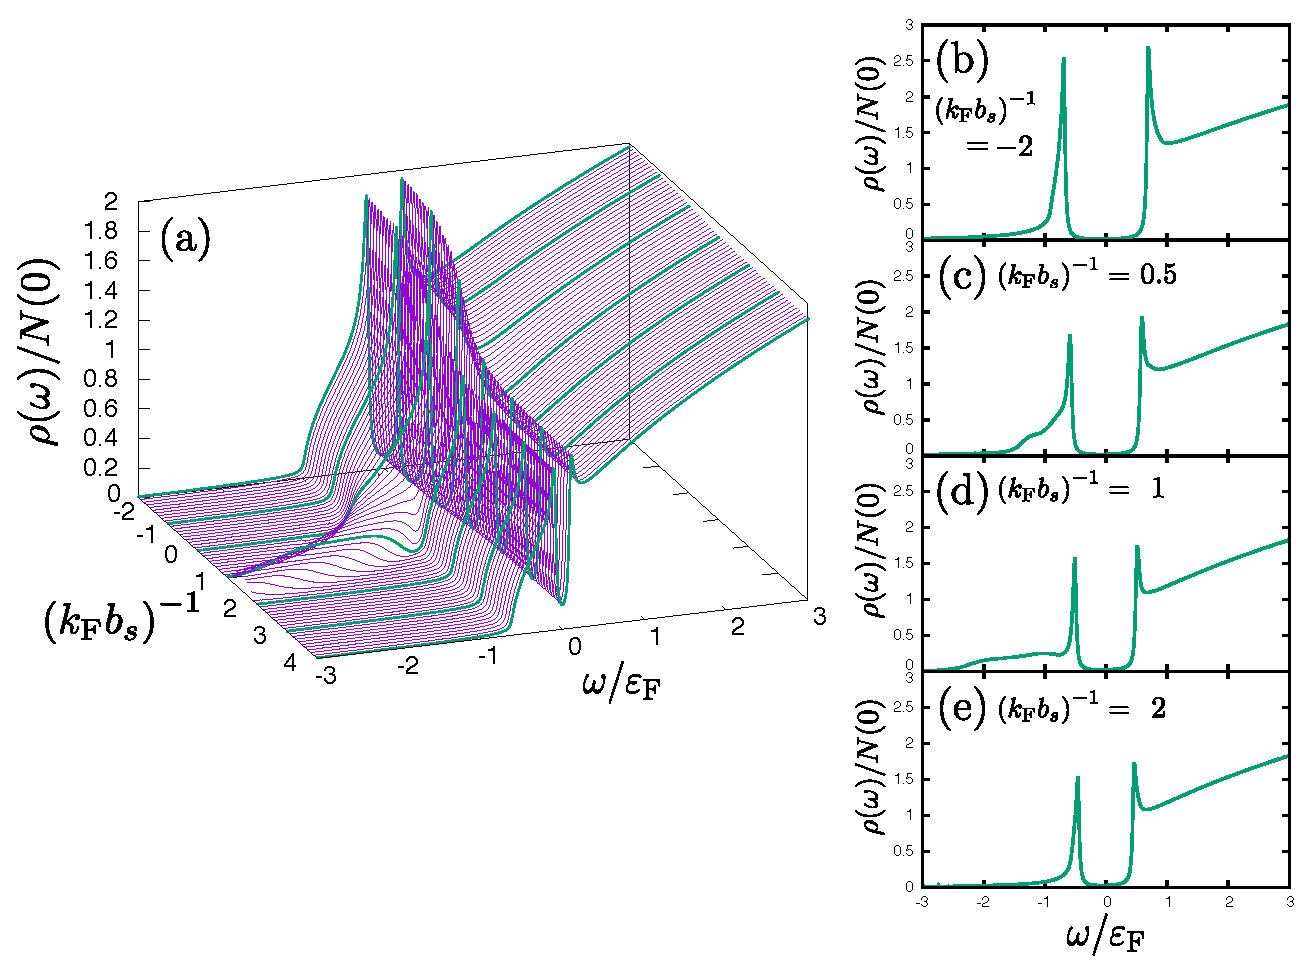
\includegraphics[width=130mm]{eps/bcsl-dos-sp-c0250-ias-10.eps}
\caption{超流動状態密度の不純物散乱強度依存性。$\lc=0.25$ で弱結合 BCS 領域($\askfi=-1$)の結果。}
\label{fig:bcsl:imp:bcsld-sp-c0250ias-10}
\end{figure}
\begin{figure}[t]
\centering
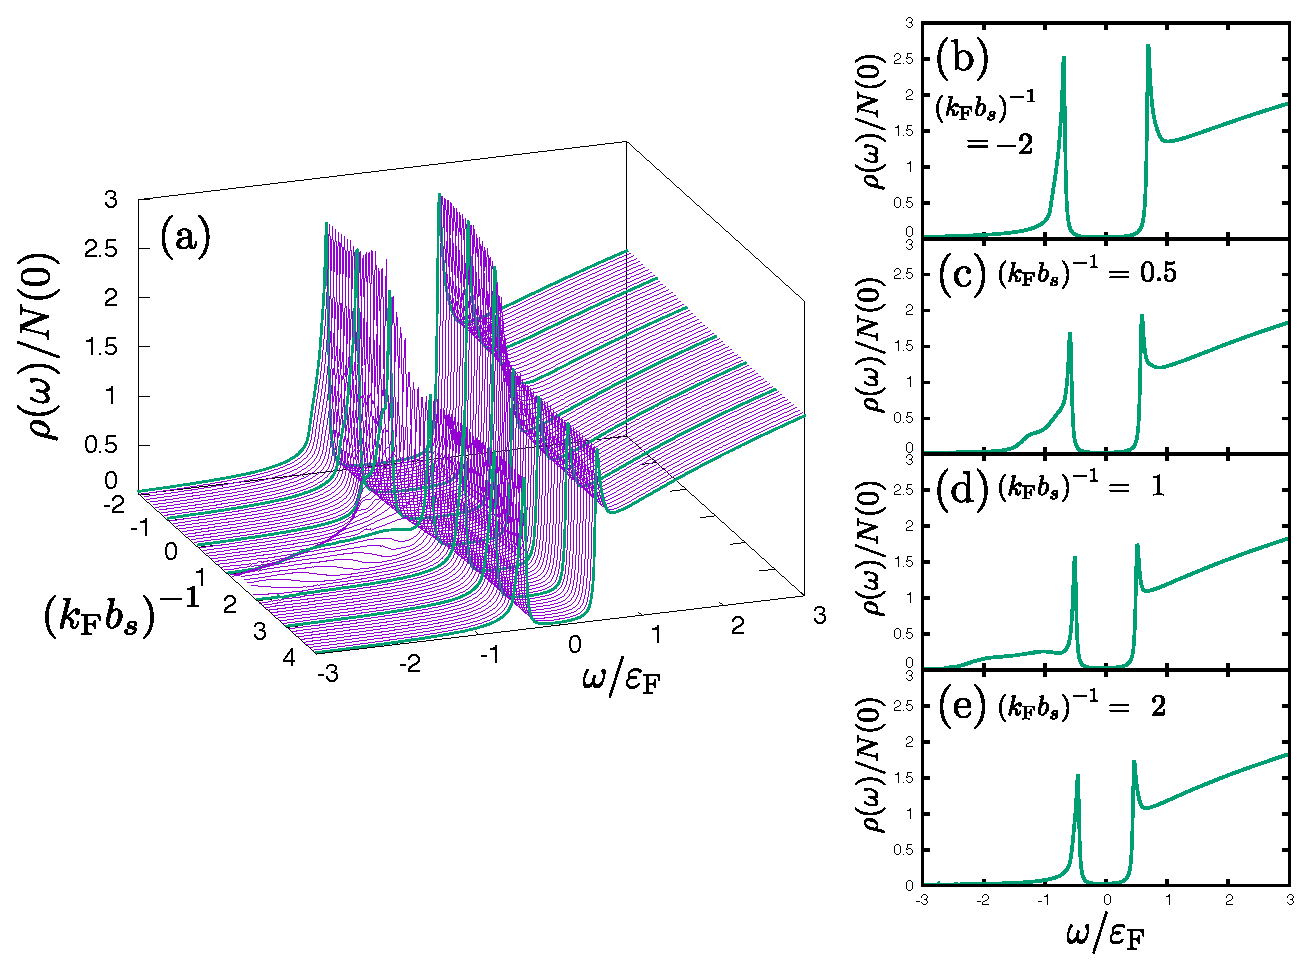
\includegraphics[width=130mm]{eps/bcsl-dos-sp-c0250-ias000.eps}
\caption{図 \ref{fig:bcsl:imp:bcsld-sp-c0250ias-10} と同じ($\lc=0.25$)であるがユニタリ極限($\askfi=0$)の結果。}
\label{fig:bcsl:imp:bcsld-sp-c0250ias000}
\end{figure}



図 \ref{fig:bcsl:imp:bcsld-sp-c0250ias-10} $\sim$ \ref{fig:bcsl:imp:bcsld-sp-c0250ias+10} は、超流動状態密度 $\rho(\omega)$ に対する非磁性不純物散乱強度$\left(\bskfi\right)$ 依存性である。その場合に共通しているのは各図 (c) において、不純物散乱強度が束縛状態を形成する程強くなると $\left(\bskfi>0\right)$、エネルギーが負の領域に不純物バンドが現れ、それが $\bskfi$ が大きくなるにつれ(束縛エネルギーの増大を反映し)低エネルギー側へシフトする、という点である。$\lc=0.25$ の場合、この不純物バンドには $N/2$ 個のフェルミ原子が収容できることから、この振る舞いは超流動に寄与する原子のうち半分が、不純物バンドに奪われている様子を表している。この現象が起こることで“伝導バンド”の原子数が減少、状態密度に現れるギャップ構造の幅も狭くなる。

図 \ref{fig:bcsl:imp:bcsld-sp-c0250ias-10}、\ref{fig:bcsl:imp:bcsld-sp-c0250ias000} ではギャップの両端に BCS 状態の特徴であるいわゆる“コヒーレンスピーク”と呼ばれるピーク構造が見られるが、図 \ref{fig:bcsl:imp:bcsld-sp-c0250ias+10} の不純物散乱が弱い領域 $\bskfi<0$ には見られない。これはこの領域の化学ポテンシャルが負であるため、正常相の状態密度は、
\beq
N(\omega) \propto \sqrt{\omega-|\cpt|} \theta(\omega- | \cpt|),
\eeq
のようにすでにギャップが開き、$\omega=0$ で状態がなくなることに起因する。ところが、$\bskfi>0$ で不純物バンドが自由フェルミ原子気体の状態密度の下に形成され始めると(図 \ref{fig:bcsl:imp:bcsld-sp-c0250ias-10})、$\omega=0$ の状態が有限となり、強結合領域でありながら状態がフェルミ面が存在する弱結合 BCS 領域に似てくるため、図 \ref{fig:bcsl:imp:bcsld-sp-c0250ias+10} にみられるように、ギャップの両端にコヒーレンスピークが生じる。しかし、$\bskfi\gg1$ となり不純物バンドのエネルギーが十分低くなり無視できるようになると、状況は $N/2$ 粒子の強結合フェルミ原子気体に帰着、コヒーレンスピークは消失する。

\clearpage
\begin{figure}[t]
\centering
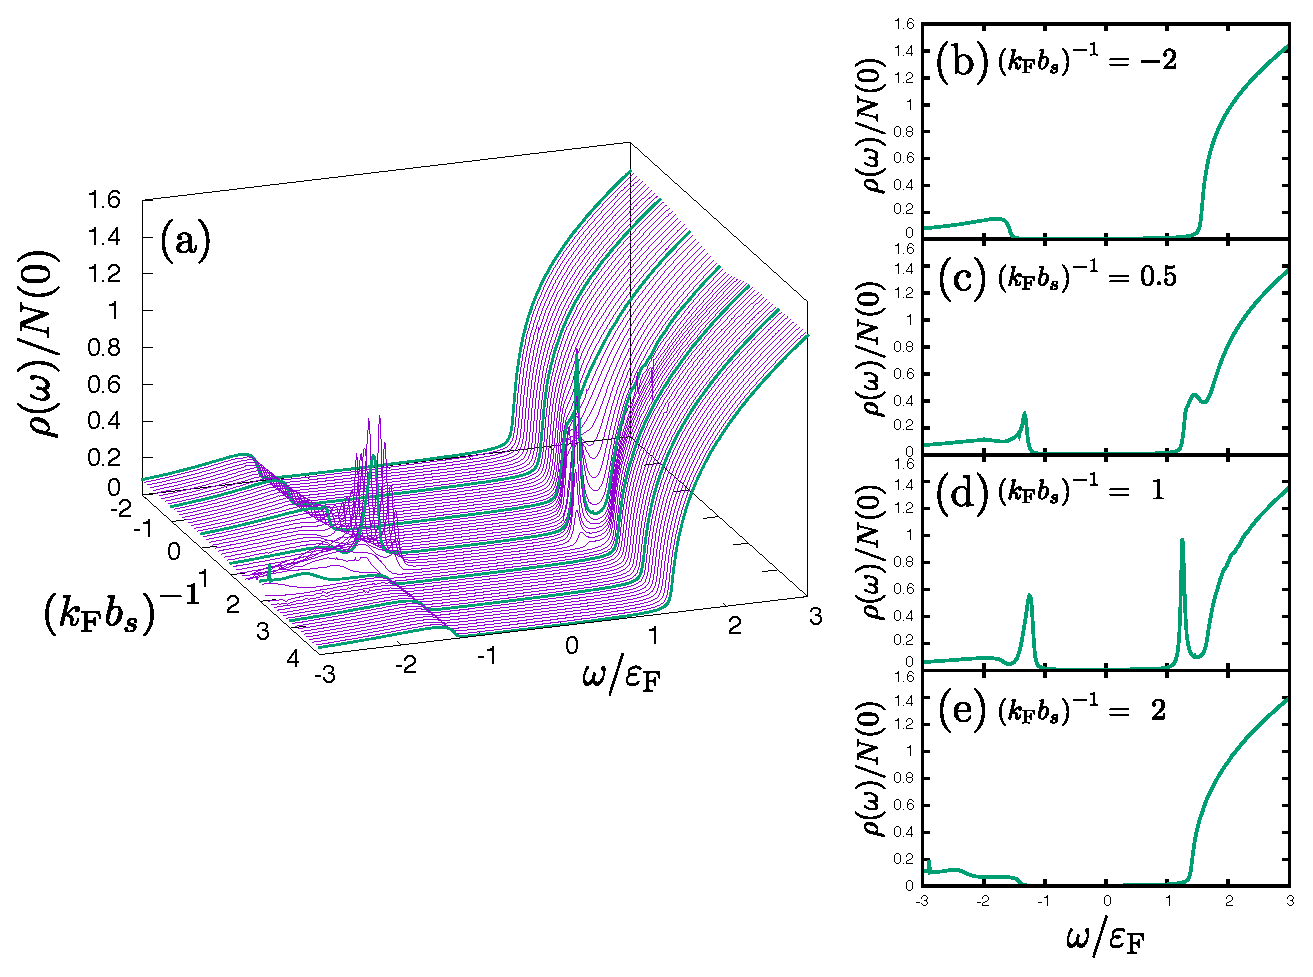
\includegraphics[width=130mm]{eps/bcsl-dos-sp-c0250-ias+10.eps}
\caption{図 \ref{fig:bcsl:imp:bcsld-sp-c0250ias-10} と同じ($\lc=0.25$)であるが強結合 BEC 領域($\askfi=1$)の結果。}
\label{fig:bcsl:imp:bcsld-sp-c0250ias+10}
\end{figure}

この現象は超流動状態が不純物散乱効果で消失する $\lc=0.5$ の場合にも見られる。図 \ref{fig:bcsl:imp:bcsld-sp-c0500ias+10} (a1)-(c4) において、化学ポテンシャルが正でフェルミ面が常流動相で存在する $\askfi=-1, 0$ のとき(図 \ref{fig:bcsl:imp:bcsld-sp-c0500ias+10}(a1)-(a4),(b1)-(b4))では、散乱強度が強くなるにつれ、$\del$ が減少、それに伴って超流動状態密度のギャップ端に現れるコヒーレンスピークの構造も顕著ではなくなる。これに対し、化学ポテンシャルが負である図 \ref{fig:bcsl:imp:bcsld-sp-c0500ias+10} (c1)-(c4) $\left(\askfi=1\right)$ では、$\bskfi<0$ ではコヒーレンスピークがなかったものが、$\bskfi>0$ で不純物束縛状態が形成され、バンドの底の構造に影響が出始めるとコヒーレンスピークが逆に顕著になってくる。この現象は、$\bskfi=1.1$ で $\del$ が消失することを除けば $\lc=0.25$ の BEC 領域での結果(図 \ref{fig:bcsl:imp:bcsld-sp-c0250ias+10})と同じである。

\begin{figure}[t]
\centering
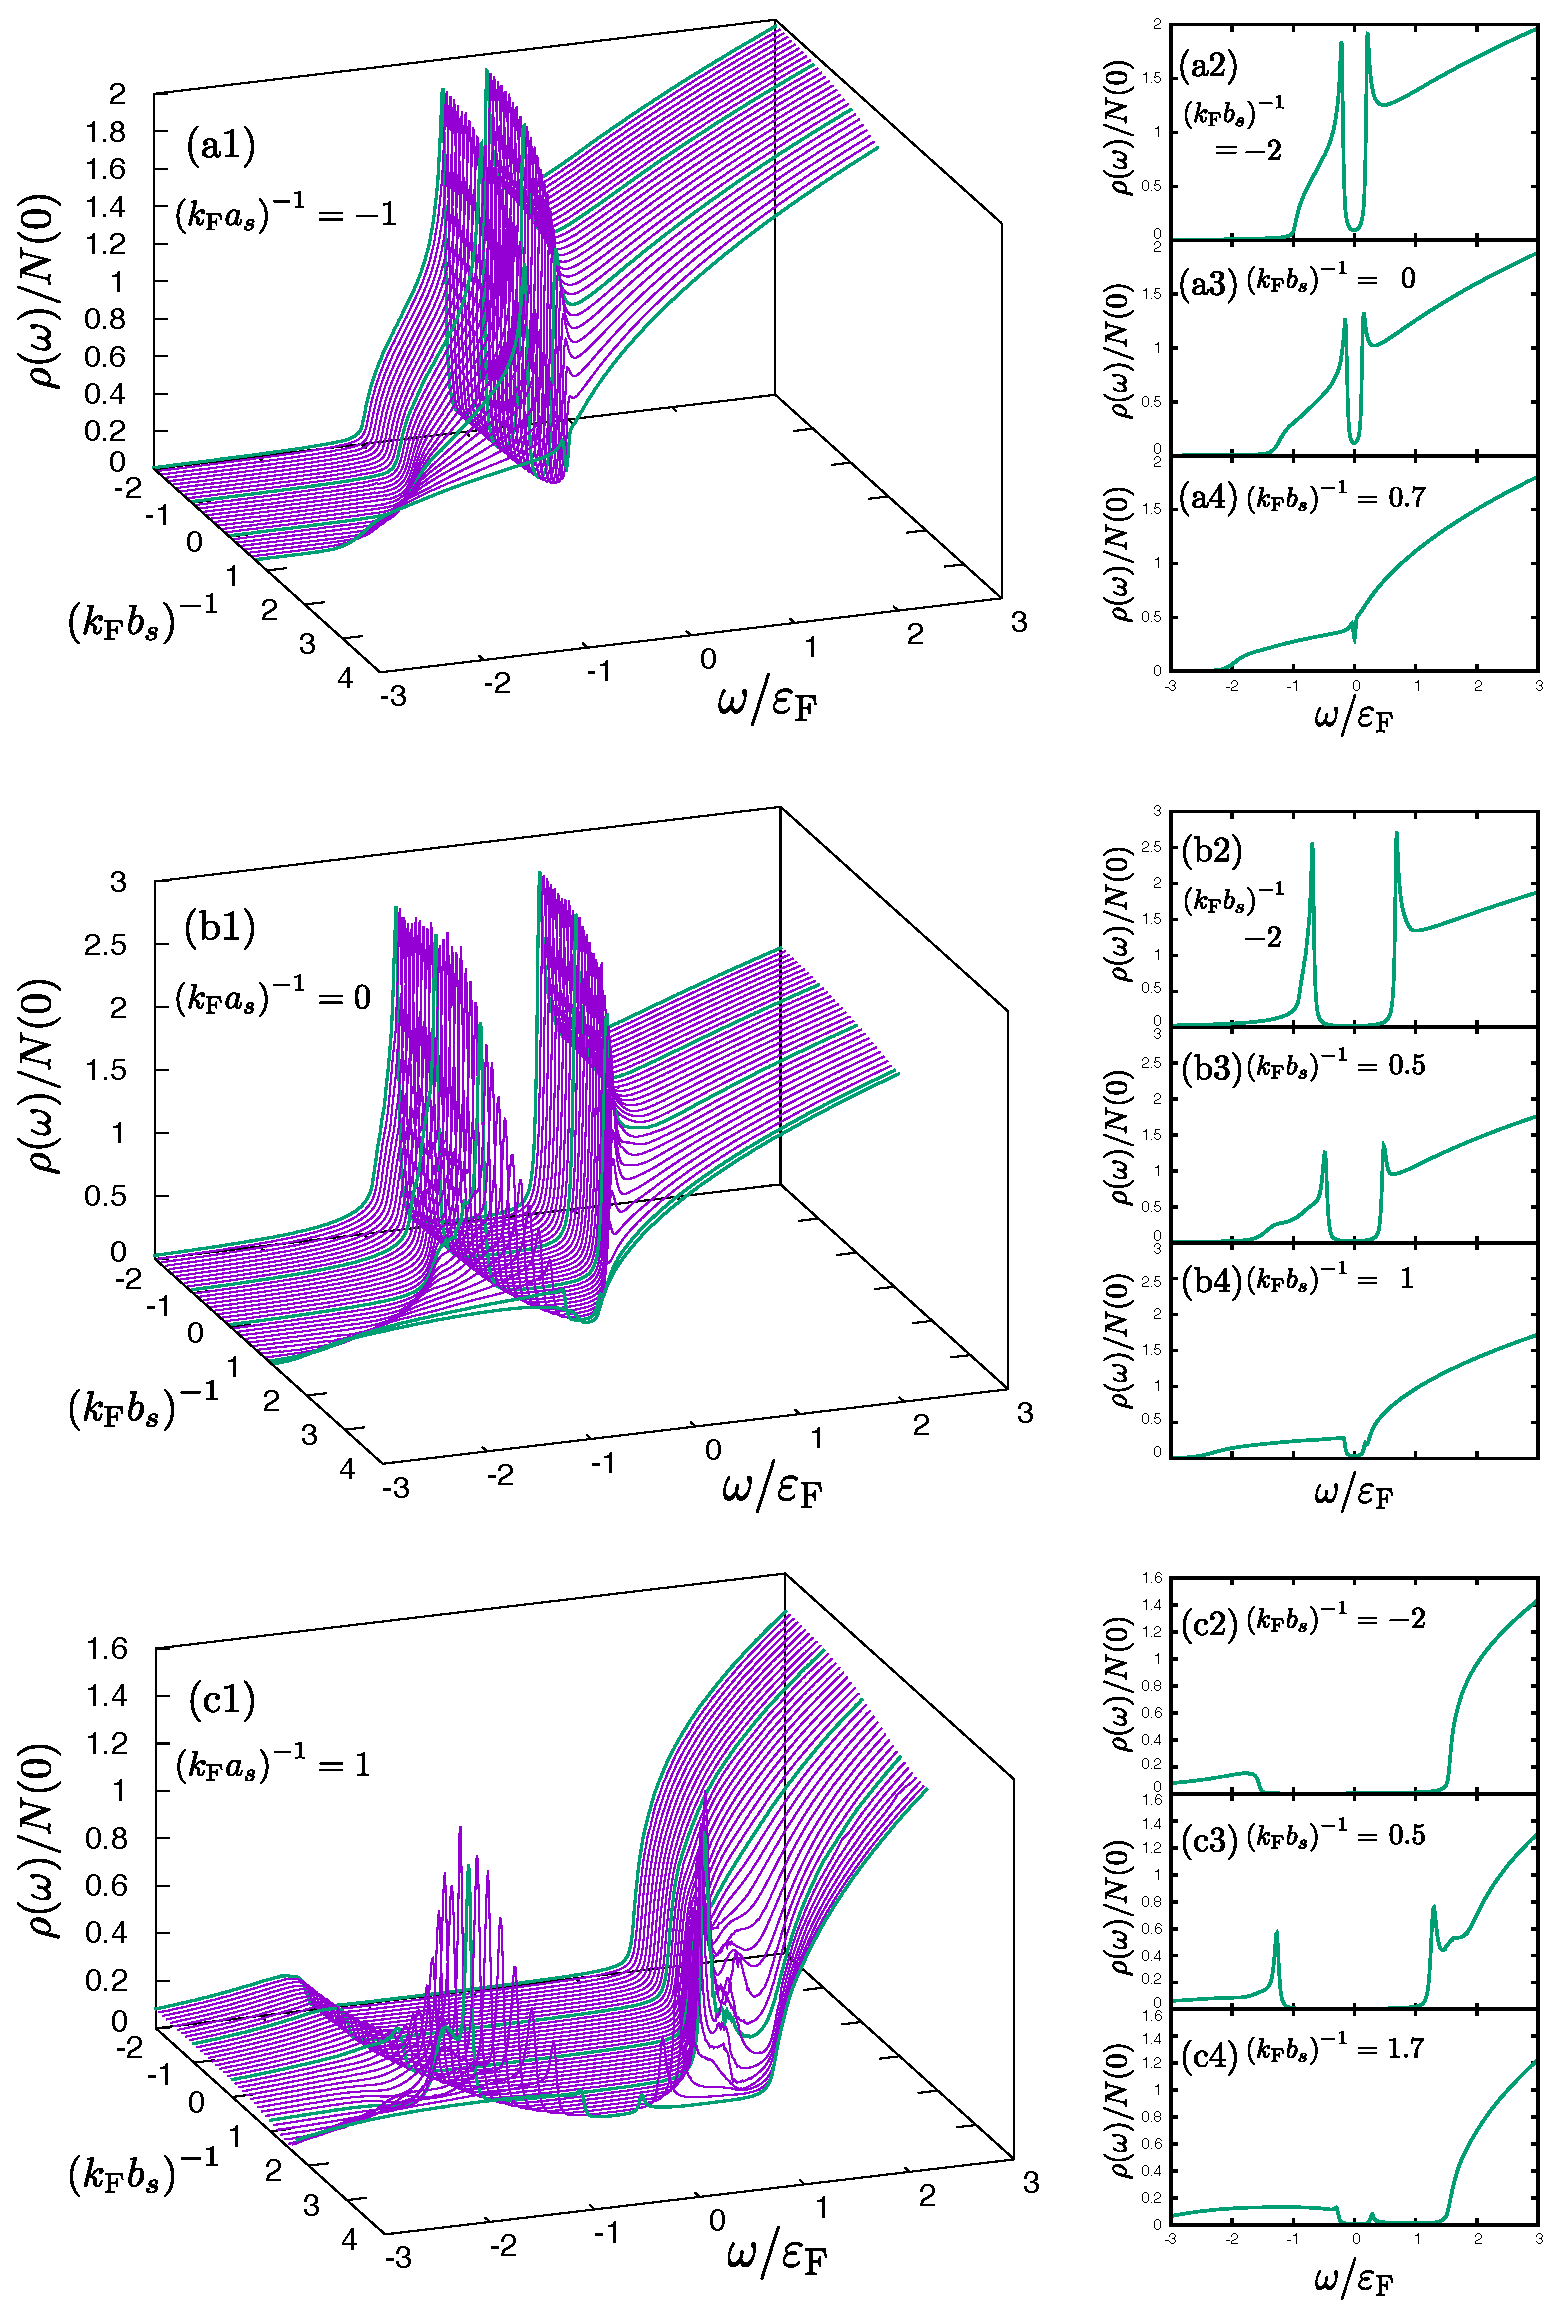
\includegraphics[width=100mm]{eps/sp-c0500-sample2.eps}
\caption{不純物濃度 $\lc=0.5$ での超流動状態における状態密度 $\rho(\omega)$ の不純物強度 $\bskfi$ 依存性。(a1)-(a4) はBCS 側($\askfi=-1$)。(b1)-(b4) はユニタリ極限($\askfi=0$)。(c1)-(c4) はBEC 側($\askfi=1$)。各図の 2-4 は、典型的な散乱強度 $\bskfi$ に対する結果をプロットしてある。特に、(a4)、(b4)、(c4)の図は、超流動秩序が消える直前の状態密度である。}
\label{fig:bcsl:imp:bcsld-sp-c0500ias+10}
\end{figure}

\clearpage

\s{1 粒子スペクトル強度に対する不純物効果}\label{sec:bcsl:bsi:spectl}


\ref{sec:bcsl:dos-imp}、\ref{sec:bcsl:bsi:iasvsibs} 節では、 1 粒子状態密度、
\beq
\rho(\omega)=-\frac{1}{\pi} \im \sum_{\bp} \bm{G}^{11}_{\bp}(i\omega_n \to \omega+i\delta),
\eeq
に現れる不純物効果を考えたが、ここでは運動量分解された状態密度である 1 粒子スペクトル強度、
\beq
A_{\bp}(\omega) = - \frac{1}{\pi} \im \bm{G}^{11}_{\bp}(i\omega_n \to \omega+i\delta),
\eeq
について考える。この量は 1 粒子状態密度と次式でつながっている。
\beq
\rho(\omega) &= \sum_{\bp} A_{\bp}(\omega)\notag\\
& = \frac{1}{32 \pi^2} \int^{\infty}_{0} \diff p \ p^2 A_{\bp}(\omega).
\eeq


\begin{figure}[t]
\centering
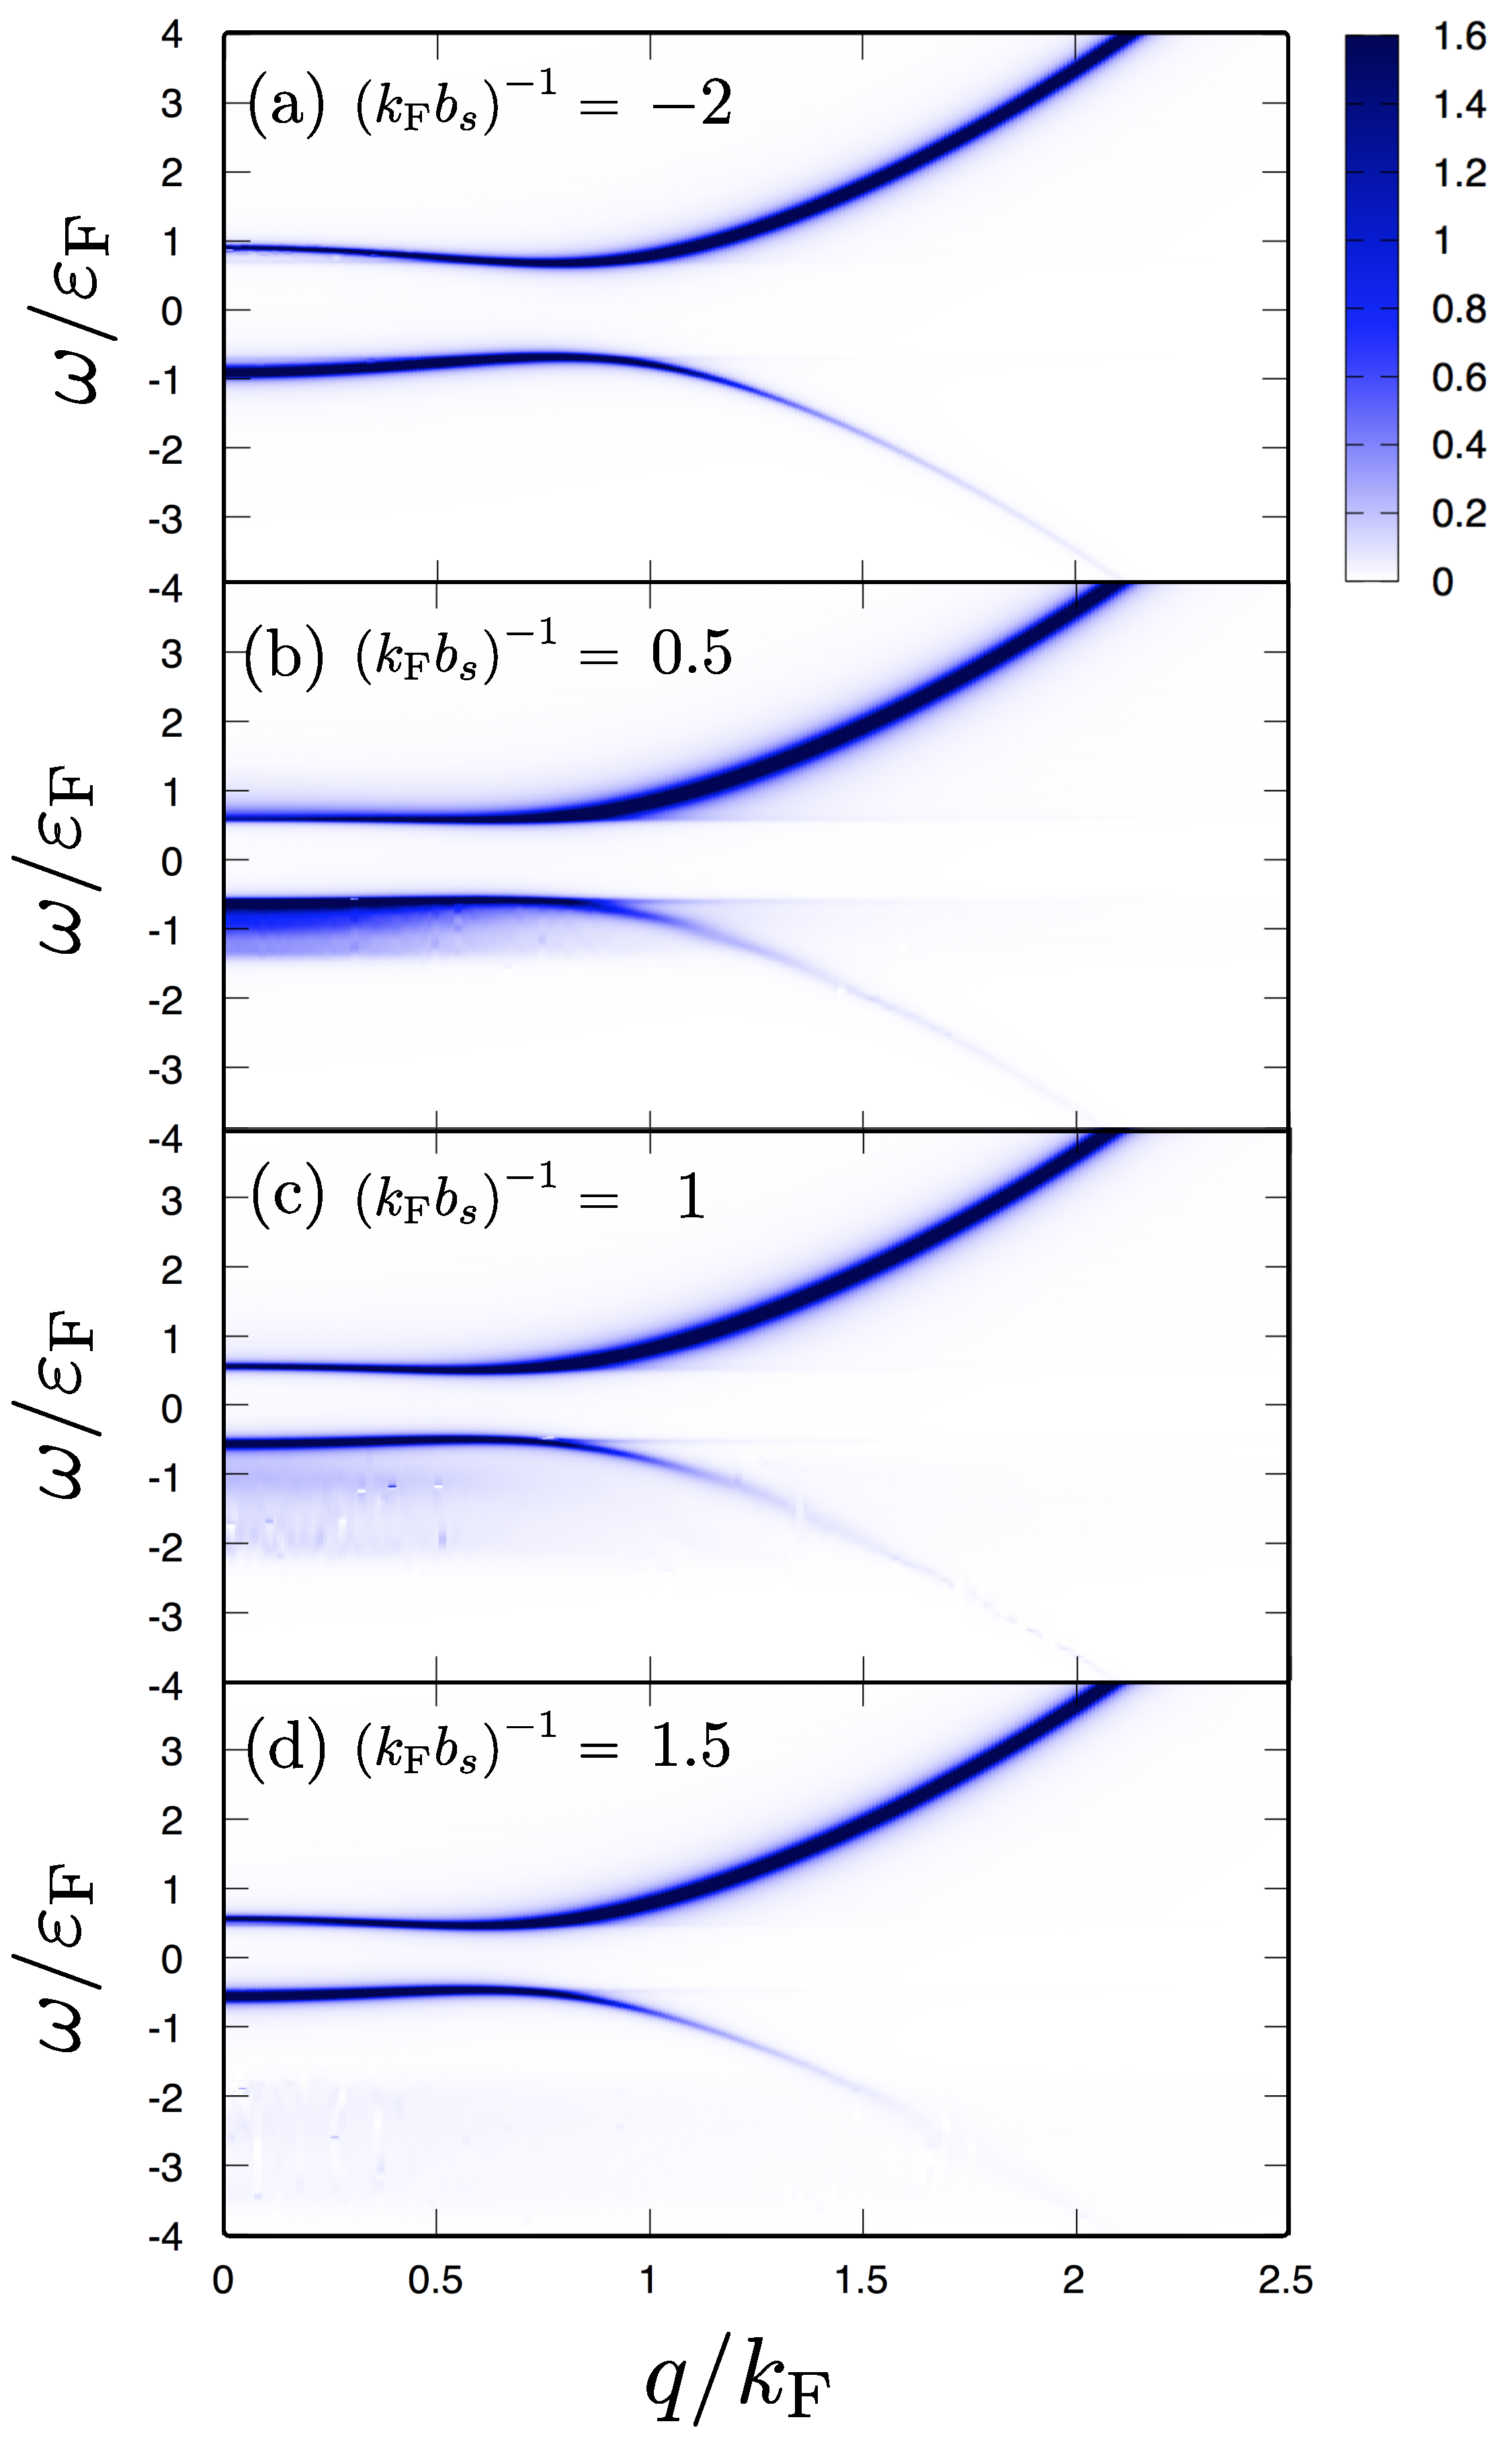
\includegraphics[width=90mm]{eps/bcsl-spec-c0250.eps}
\caption{$\overline{c}=0.25$、ユニタリ極限 $\askfi=0$ の超流動一粒子スペクトルの不純物散乱長 $\bskfi$ 依存性。}
\label{fig:bcsl:imp:map-c0250}
\end{figure}
\begin{figure}[t]
\centering
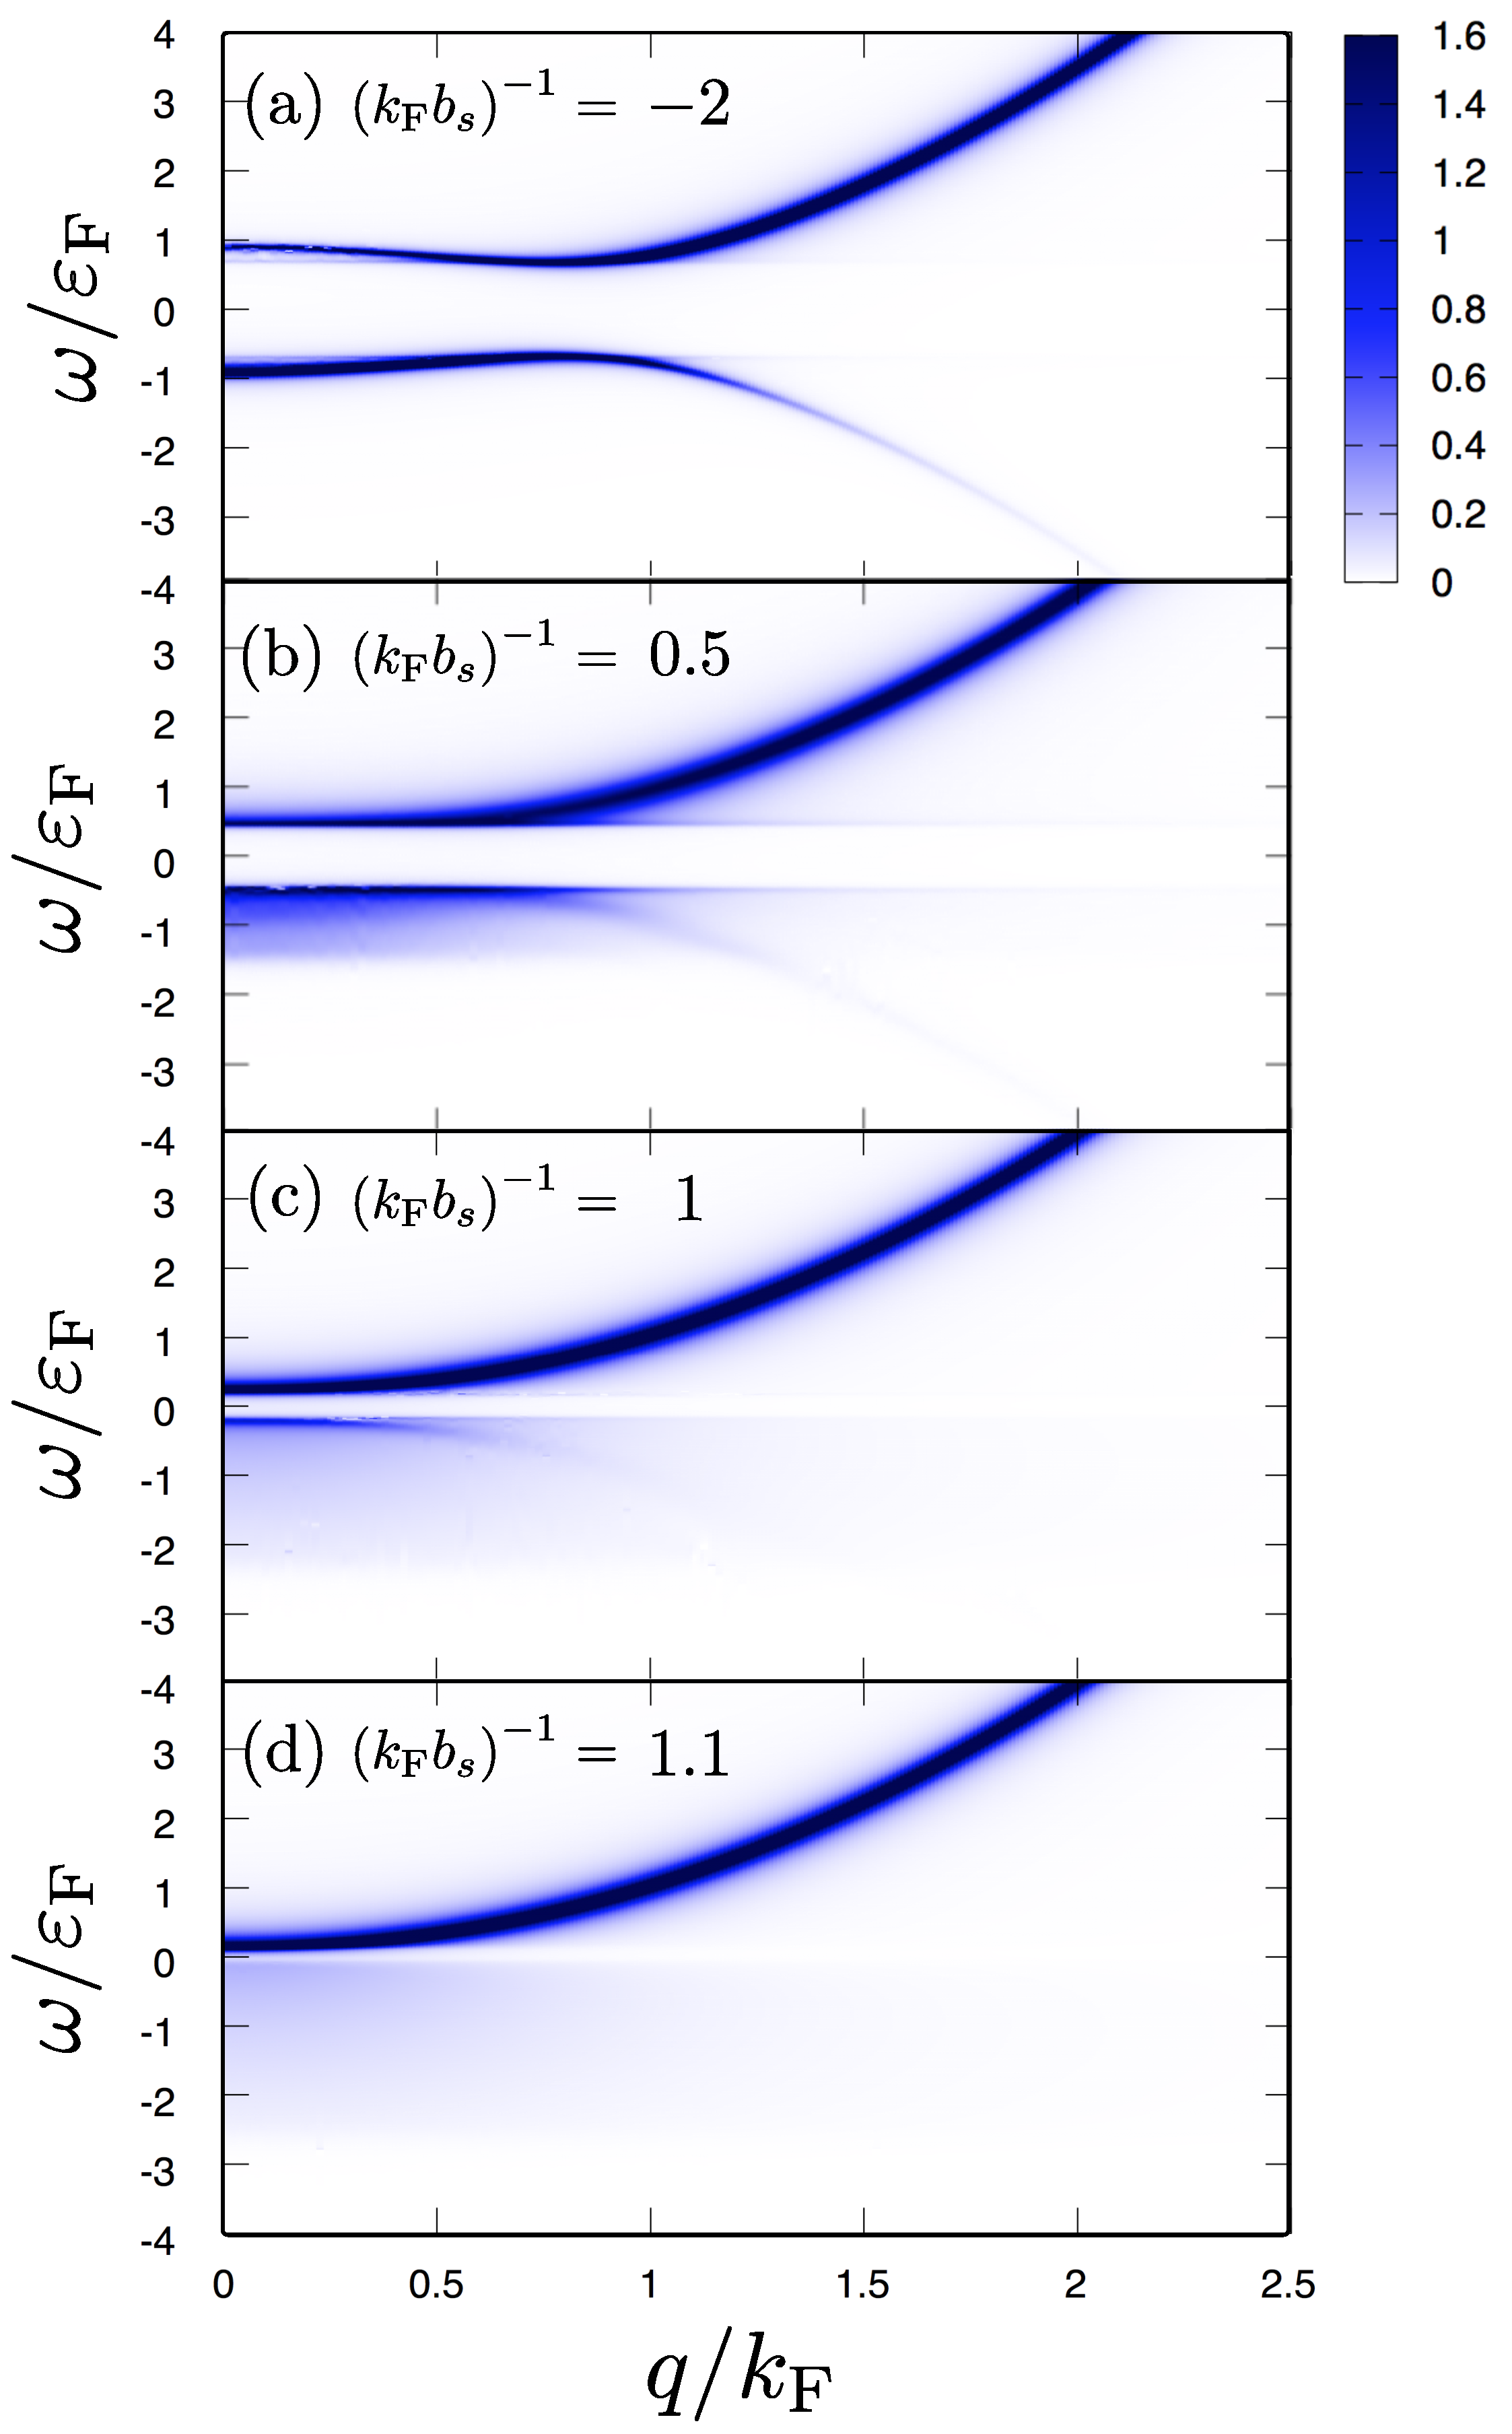
\includegraphics[width=90mm]{eps/bcsl-spec-c0500.eps}
\caption{$\overline{c}=0.5$、ユニタリ極限 $\askfi=0$  の超流動一粒子スペクトルの不純物散乱長 $\bskfi$ 依存性。}
\label{fig:bcsl:imp:map-c0500}
\end{figure}
\begin{figure}[t]
\centering
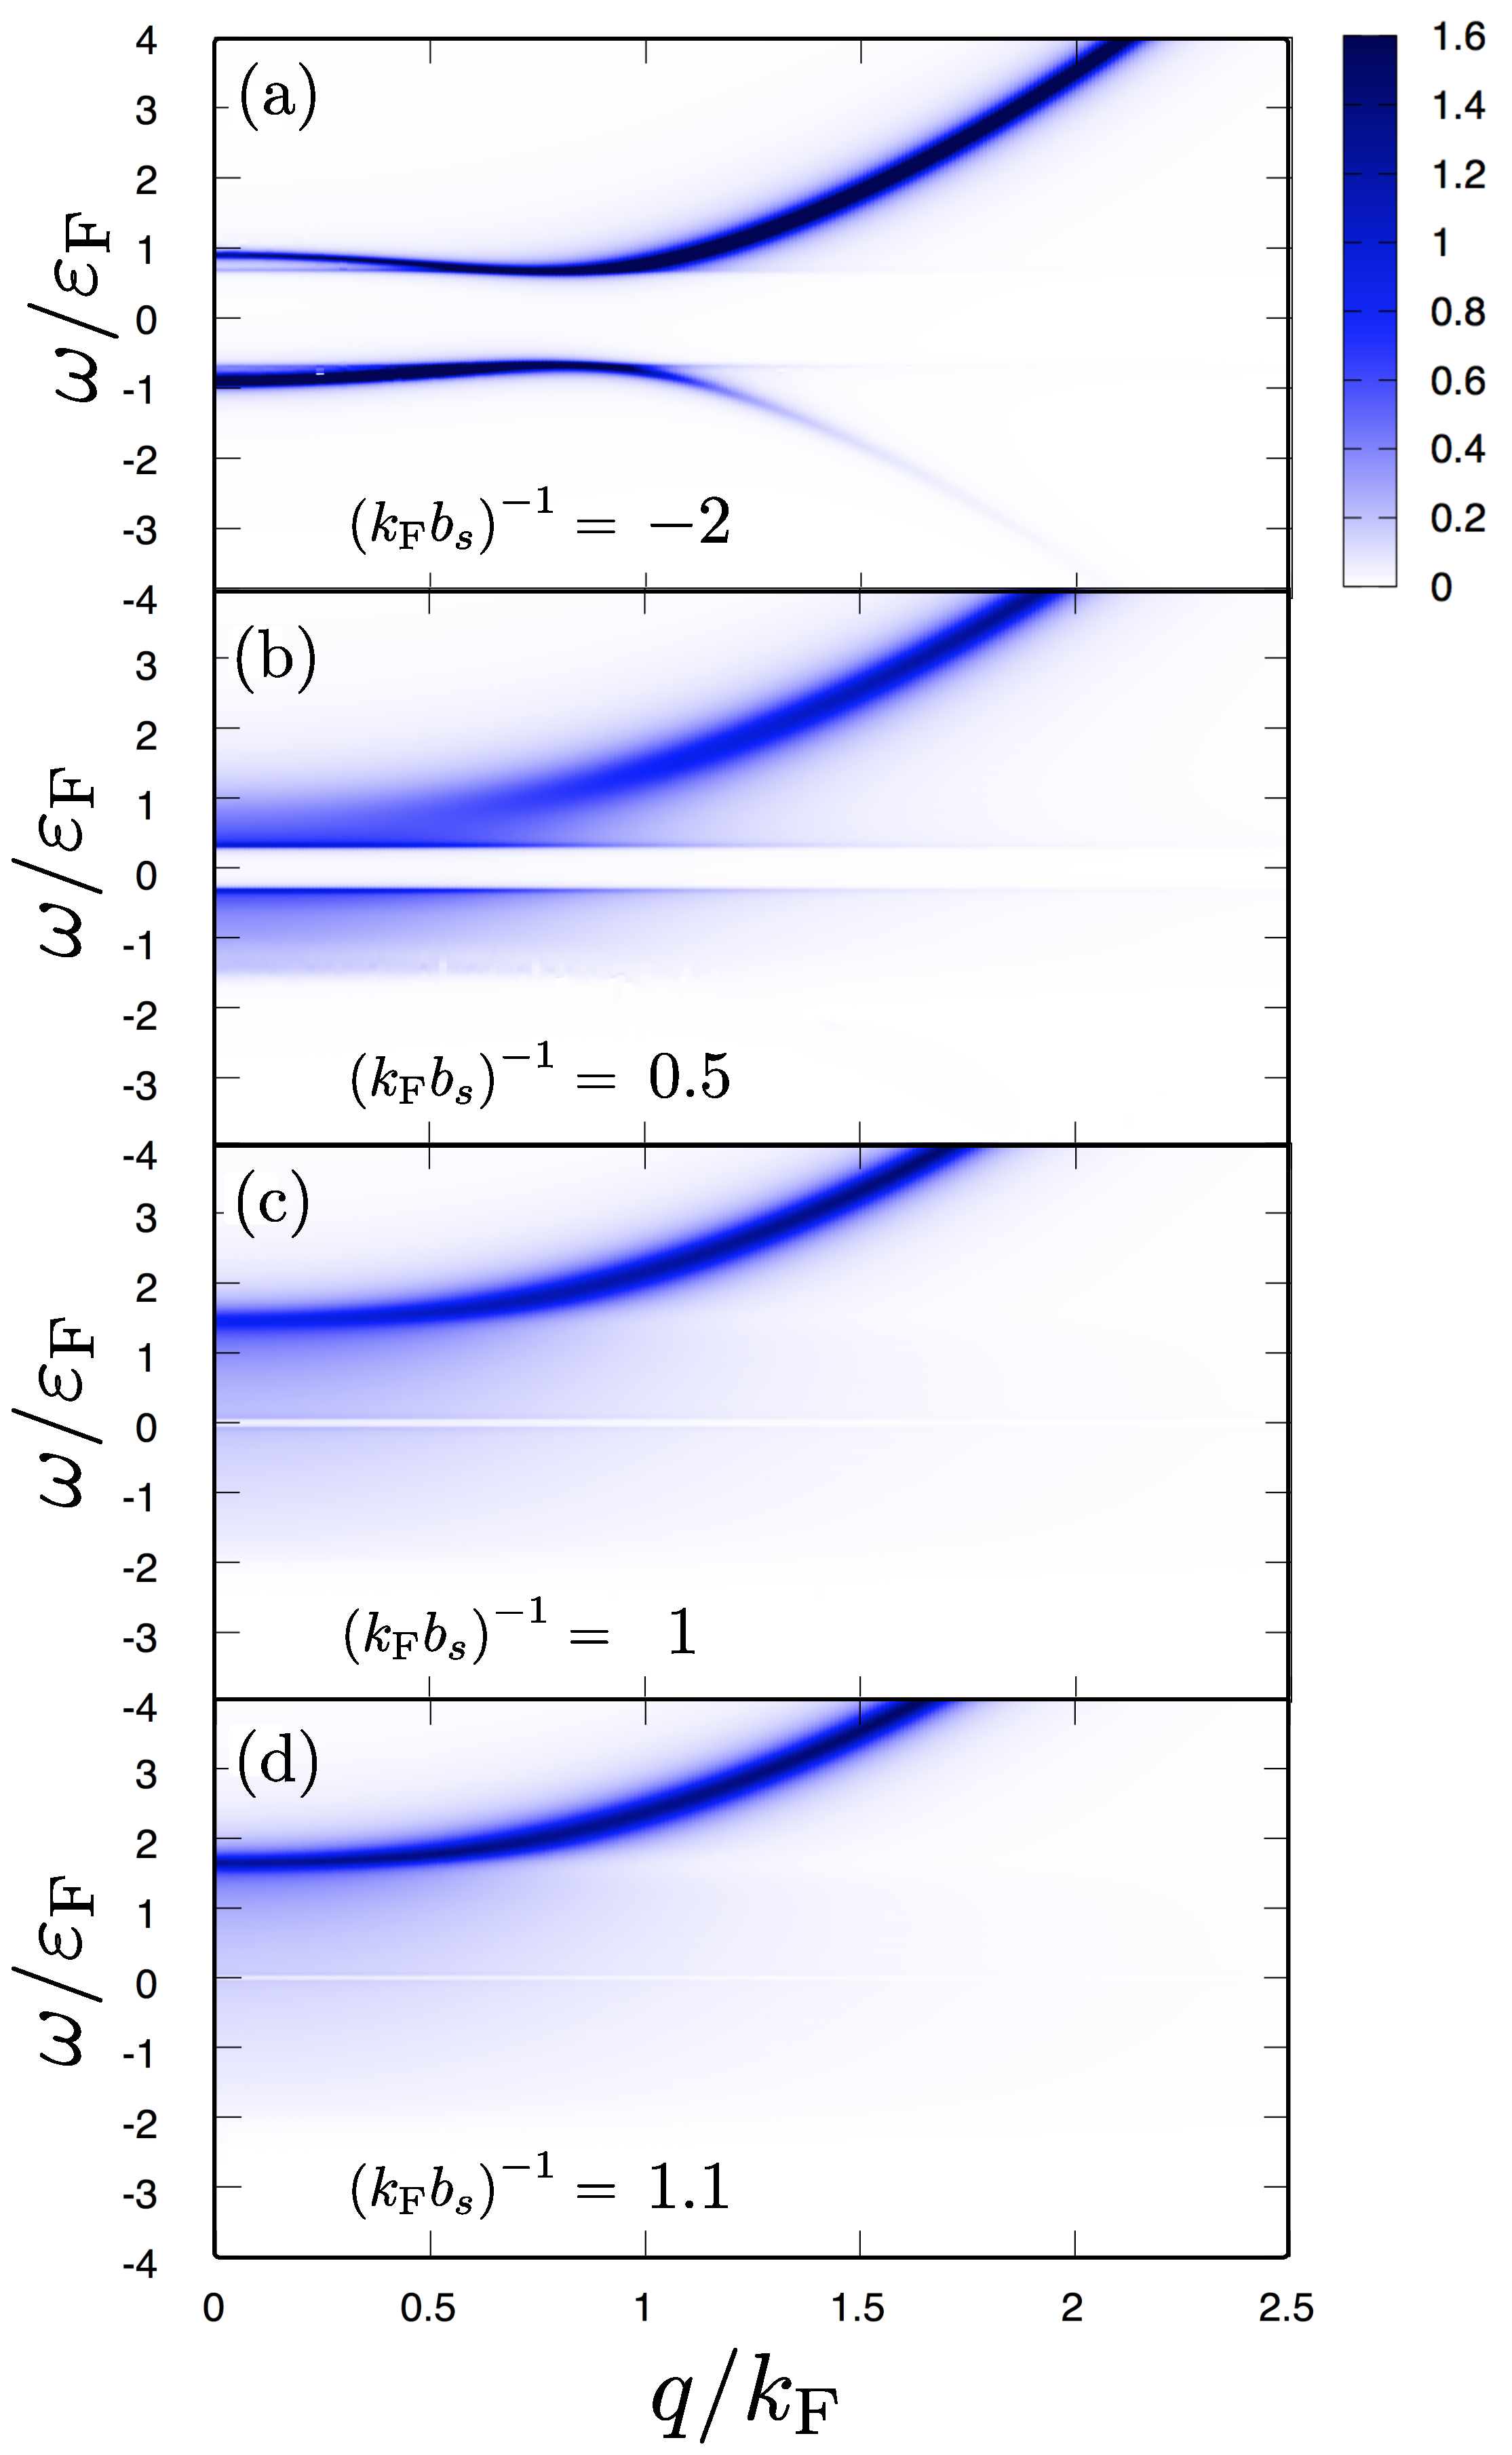
\includegraphics[width=90mm]{eps/bcsl-spec-c1000.eps}
\caption{$\overline{c}=1$、ユニタリ極限 $\askfi=0$ の超流動一粒子スペクトルの不純物散乱長 $\bskfi$ 依存性。}
\label{fig:bcsl:imp:map-c1000}
\end{figure}


図 \ref{fig:bcsl:imp:map-c0250} $\sim$ \ref{fig:bcsl:imp:map-c1000} に 3 種類の不純物濃度における 1 粒子スペクトル強度 $A_{\bp}(\omega)$ の不純物散乱強度依存性を示す。 $\lc=0.25 (<0.5)$ の場合、(a) では不純物散乱が弱いためスペクトル構造はほとんど BCS 理論の場合に等しい。超流動秩序パラメータ $\del$、化学ポテンシャル $\cpt$ とするとスペクトルのピークはボゴリューボフ分散、
\beq
E^{\pm}_{\bp} = \pm \sqrt{\left(\ken_p-\cpt\right)^2 + \del^2},
\eeq
に沿っている。不純物散乱強度 $\bskfi$ が大きくなる(図 \ref{fig:bcsl:imp:map-c0250} (b)) になると、準粒子励起が寿命を持つことを反映し、ボゴリューボフ分散がぼやけてくる。また、“不純物バンド”と“伝導バンド”の分裂が起こることを反映し、図 \ref{fig:bcsl:imp:map-c0250} (c) では、下のボゴリューボフバンドの下あたりに、ブロードなスペクトルが現れる。不純物バンドが分裂、下方にシフトして伝導バンドから完全に切り離されると、伝導バンドの方は原子数が $N/2$ となったフェルミ原子気体になるのでボゴリューボフ分散のスペクトルは再びシャープになる(ただしギャップサイズは小さくなる)。

$\lc=0.5$ の場合は、図 \ref{fig:bcsl:imp:map-c0500} に示すように不純物散乱強度 $\bskfi$ が大きくなるに従ってボゴリューボフ分散がぼやけていくとともに、$E_{\bp}^{-}$ がブロードな不純物バンドに移り変わっていく。図 \ref{fig:bcsl:imp:map-c0500} (d) では(数値計算の精度の範囲で) $\del=0$ となるが、この時は 1 粒子分散の下に不純物バンドに起因するブロードな不純物バンドが存在する状態が実現する。


$\lc=1$ の場合(図 \ref{fig:bcsl:imp:map-c1000})に示すように不純物散乱強度 $\bskfi$ が大きくなると不純物バンド内に超流動ギャップが生じるが、これは図 \ref{fig:bcsl:imp:map-c1000} (d) の $\omega=0$ 付近の狭いギャップとしてスペクトル強度 $A_{\bp}(\omega)$ に現れる。しかしこの時、図 \ref{fig:bcsl:imp:map-c1000} (a) と比べてわかるように図 \ref{fig:bcsl:imp:map-c1000} (d) の超流動ギャップの上下にボゴリューボフの分散構造は現れない。

以上、$T=0$ の結果から、非磁性不純物散乱は一般には $T=0$ 超流動秩序パラメータに影響を与えることがわかる。ただし、$\bskfi<0$ の場合、その影響は磁性不純物効果のような散乱による「対破壊」ではなく、正常相の 1 粒子状態密度が不純物散乱の影響を受けることによるものである。他方 $\bskfi>0$ で不純物とフェルミ原子とが 2 体束縛状態を形成する状況では、その束縛エネルギーがクーパー対の結合エネルギーより大きくなるとクーパー対を破壊し、不純物との束縛状態を形成するようになるため、対破壊現象が起こっているということができる。

ここでの議論は不純物とフェルミ原子との相互作用は引力であることを前提としているが、$\bskfi\gg 1$ で不純物バンドが完全に“伝導バンド”から切り離された状況は伝導バンドに関しては $\bs>0$ より斥力の状況となる。この時、$\lc<0.5$ であれば伝導バンドには不純物に束縛されなかったフェルミ原子が占有することになり、これらはもはや不純物と束縛状態を作ることはないので、不純物散乱の超流動状態への影響はほとんどない。




\s{超流動転移温度に対する不純物効果}\label{sec:bcsl:con}

\begin{figure}[t]
\centering
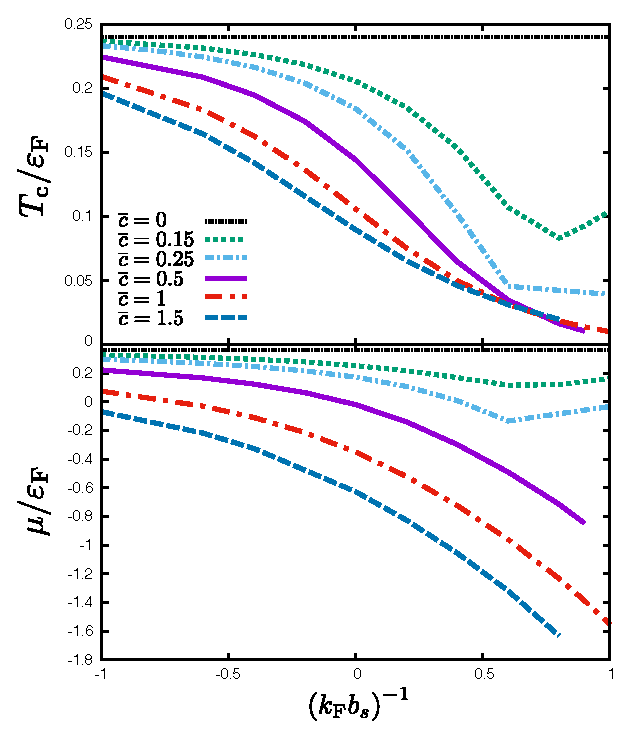
\includegraphics[width=90mm]{eps/tma-cpt-all.eps}
\caption{ユニタリー極限 $\askfi=0$ における (a) 超流動転移温度 $\tc$ と (b)  化学ポテンシャル $\cpt (\tc)$ 。}
\label{fig:bcsl:con:tma-all}
\end{figure}



\begin{figure}[t]
\centering
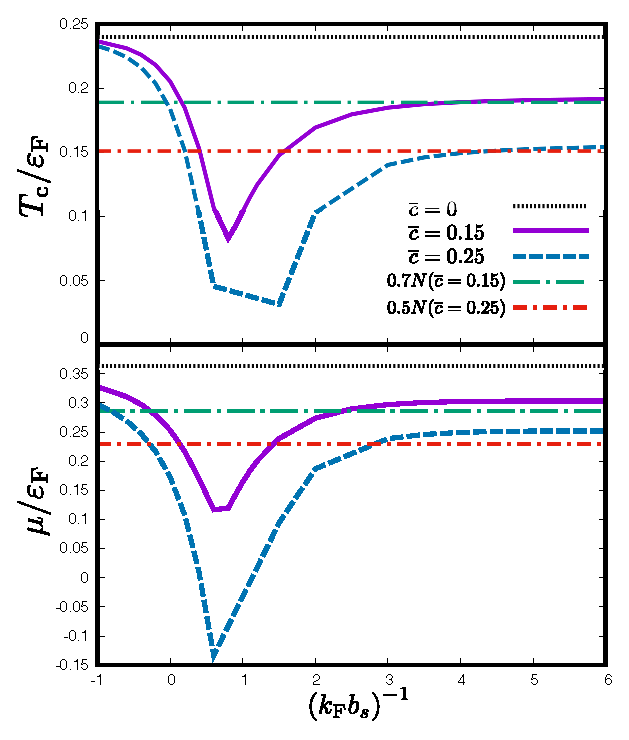
\includegraphics[width=90mm]{eps/tma-cpt-large.eps}
\caption{ユニタリー極限 $\askfi=0$ における (a) 超流動転移温度 $\tc$ と (b) 化学ポテンシャル $\cpt(\tc)$ の不純物濃度 $\overline{c}=0.15,\ 0.25$ について不純物散乱強度依存性をプロットしている。また $(1-2\lc)N$ 粒子の純粋系における値も図中に示した。}
\label{fig:bcsl:con:tma-wide}
\end{figure}

\begin{figure}[t]
\centering
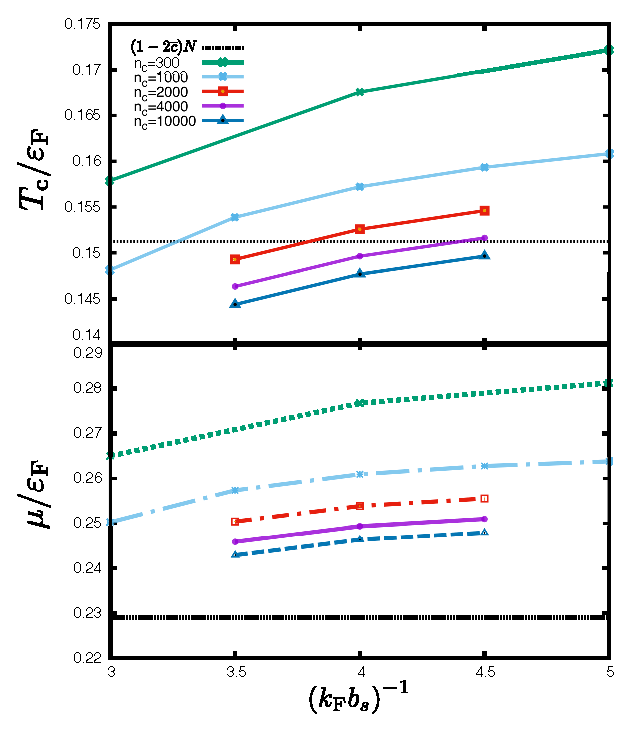
\includegraphics[width=90mm]{eps/tma-cpt-cut.eps}
\caption{ユニタリー極限 $\askfi=0$ における超流動転移温度 $\tc$ と (b) 化学ポテンシャル $\cpt(\tc)$ のフェルミオンの松原周波数のカットオフ $n_{\text{c}}$ 依存性。$(1-2\lc)N$ 粒子の純粋系における値も図中に示した。}
\label{fig:bcsl:con:tma-cut}
\end{figure}



図 \ref{fig:bcsl:con:tma-all} はユニタリ極限における超流動転移温度 $\tc$、および、化学ポテンシャル $\cpt$ に対する不純物散乱強度依存性である。この結果は、\ref{sec:form:tmat} 節の式 (\ref{eq:form:ham:sctma}), (\ref{eq:form:tma:gimp}), (\ref{eq:form:tma:gall})-(\ref{eq:form:tma:piimp}) を自己無撞着に解いて得られたものである。

不純物濃度 $\lc=0.5$ の場合、$T=0$ では$\bskfi=1.1$ で、超流動が消失 $\del=0$ したが、それを反映し、$\tc$ も $\bskfi=1$ に近づくと急速に減少する。今の計算では松原周波数の和を取るため、完全に $T=0$ とする計算はできず、$\lc=0.5$ での $\tc$ が完全に 0 になるところまでは数値的に確認できないが、 $\bskfi\gg1$ では全フェルミ原子が不純物に束縛されることを考慮すると、最終的には $\bskfi\sim1$ で$T_{\text{c}}=0$ となることが予想される。

不純物濃度が $\lc=1.0,\ 1.5\  (>0.5)$ の場合にも、$\bskfi\gtsim 0$ では $\tc$ は急速に減少するが、$\bskfi \sim 1$ で $\lc=0.5$ よりも高い $\tc$ を取るようになる。後に議論するカットオフ依存性に関係し、高い $\tc$ をとる $\bskfi$ の値は大きくなりうるが、この時は不純物バンドは“伝導バンド”から完全に分離しても部分的に占有されるだけなので $\lc=0.5$ の時と異なり $\bskfi$ が大きい領域でも $\tc$ は有限に残る。

$\lc <0.5$ の場合、$T=0$ での議論から $\bskfi \gg 1$ でも不純物に束縛されなかった $N'=N(1-2\lc)$ のフェルミ原子が超流動転移を起こすと考えられるので、$\tc>0$ となるはずである。実際 $\lc=0.15,\ 0.25$ の場合、不純物散乱強度を強くすると、$\bskfi\sim1$ で一旦は $\tc$ は減少するものの、$\bskfi\gg1$ では予想どおり一定値に近づいていく。

$\bskfi \gg 1 $ では不純物に束縛されなかった $N'=N(1-2\lc)$ 個の原子による超流動と考えられるので、この極限では不純物がない場合の$\tc$ を$\tc^{0}$ とすると、
\beq
T_c=\left(1-2 \lc\right)^{\frac{2}{3}} T_c^0,\label{eq:bcsl:con:tctc0}
\eeq
と評価できる。同様に化学ポテンシャルも不純物がない場合の値 $\cpt^0$ を用い、
\beq
\cpt=\left(1-2 \lc\right)^{\frac{2}{3}} \cpt^0,\label{eq:bcsl:con:cpcp0}
\eeq
と評価される。


図 \ref{fig:bcsl:con:tma-wide} では、$\bskfi\gg1$ での $\tc$ や $\cpt(\tc)$ は完全には式 (\ref{eq:bcsl:con:tctc0}), (\ref{eq:bcsl:con:cpcp0}) に一致していないが、これは今の数値計算が松原周波数の無限の和を有限なところで打ち切っていることに因る。すなわち、数値計算で、粒子数を本研究では、
\beq
N = 2T \sum_{\bp}\sum_{n=-n_{\rm c}}^{n_{\rm c}} \gpom e^{i \omn \delta},
\eeq
と計算している。図 \ref{fig:bcsl:con:tma-wide} では $n_{\rm c}=4000$ としているが、この $n_{\rm c}$ を変えると、より大きな $n_{\rm c}$ まで和を取ると $\tc$ は次第に式 (\ref{eq:bcsl:con:tctc0}) に $\bskfi\gg1$ で近づいていくことが見て取れる(図 \ref{fig:bcsl:con:tma-cut})。一方で、式 (\ref{eq:bcsl:con:cpcp0}) へは完全には近づかないが、これは不純物による定数的な化学ポテンシャルシフトが入っているためである。このことは次に示す、$\bskfi \simeq 3$ における状態密度がクリーン系の $N'=(1-2\lc)N$ の状態密度に漸近することから確認できる。以下では $n_{\rm c}=4000$ とする。

\begin{figure}[t]
\centering
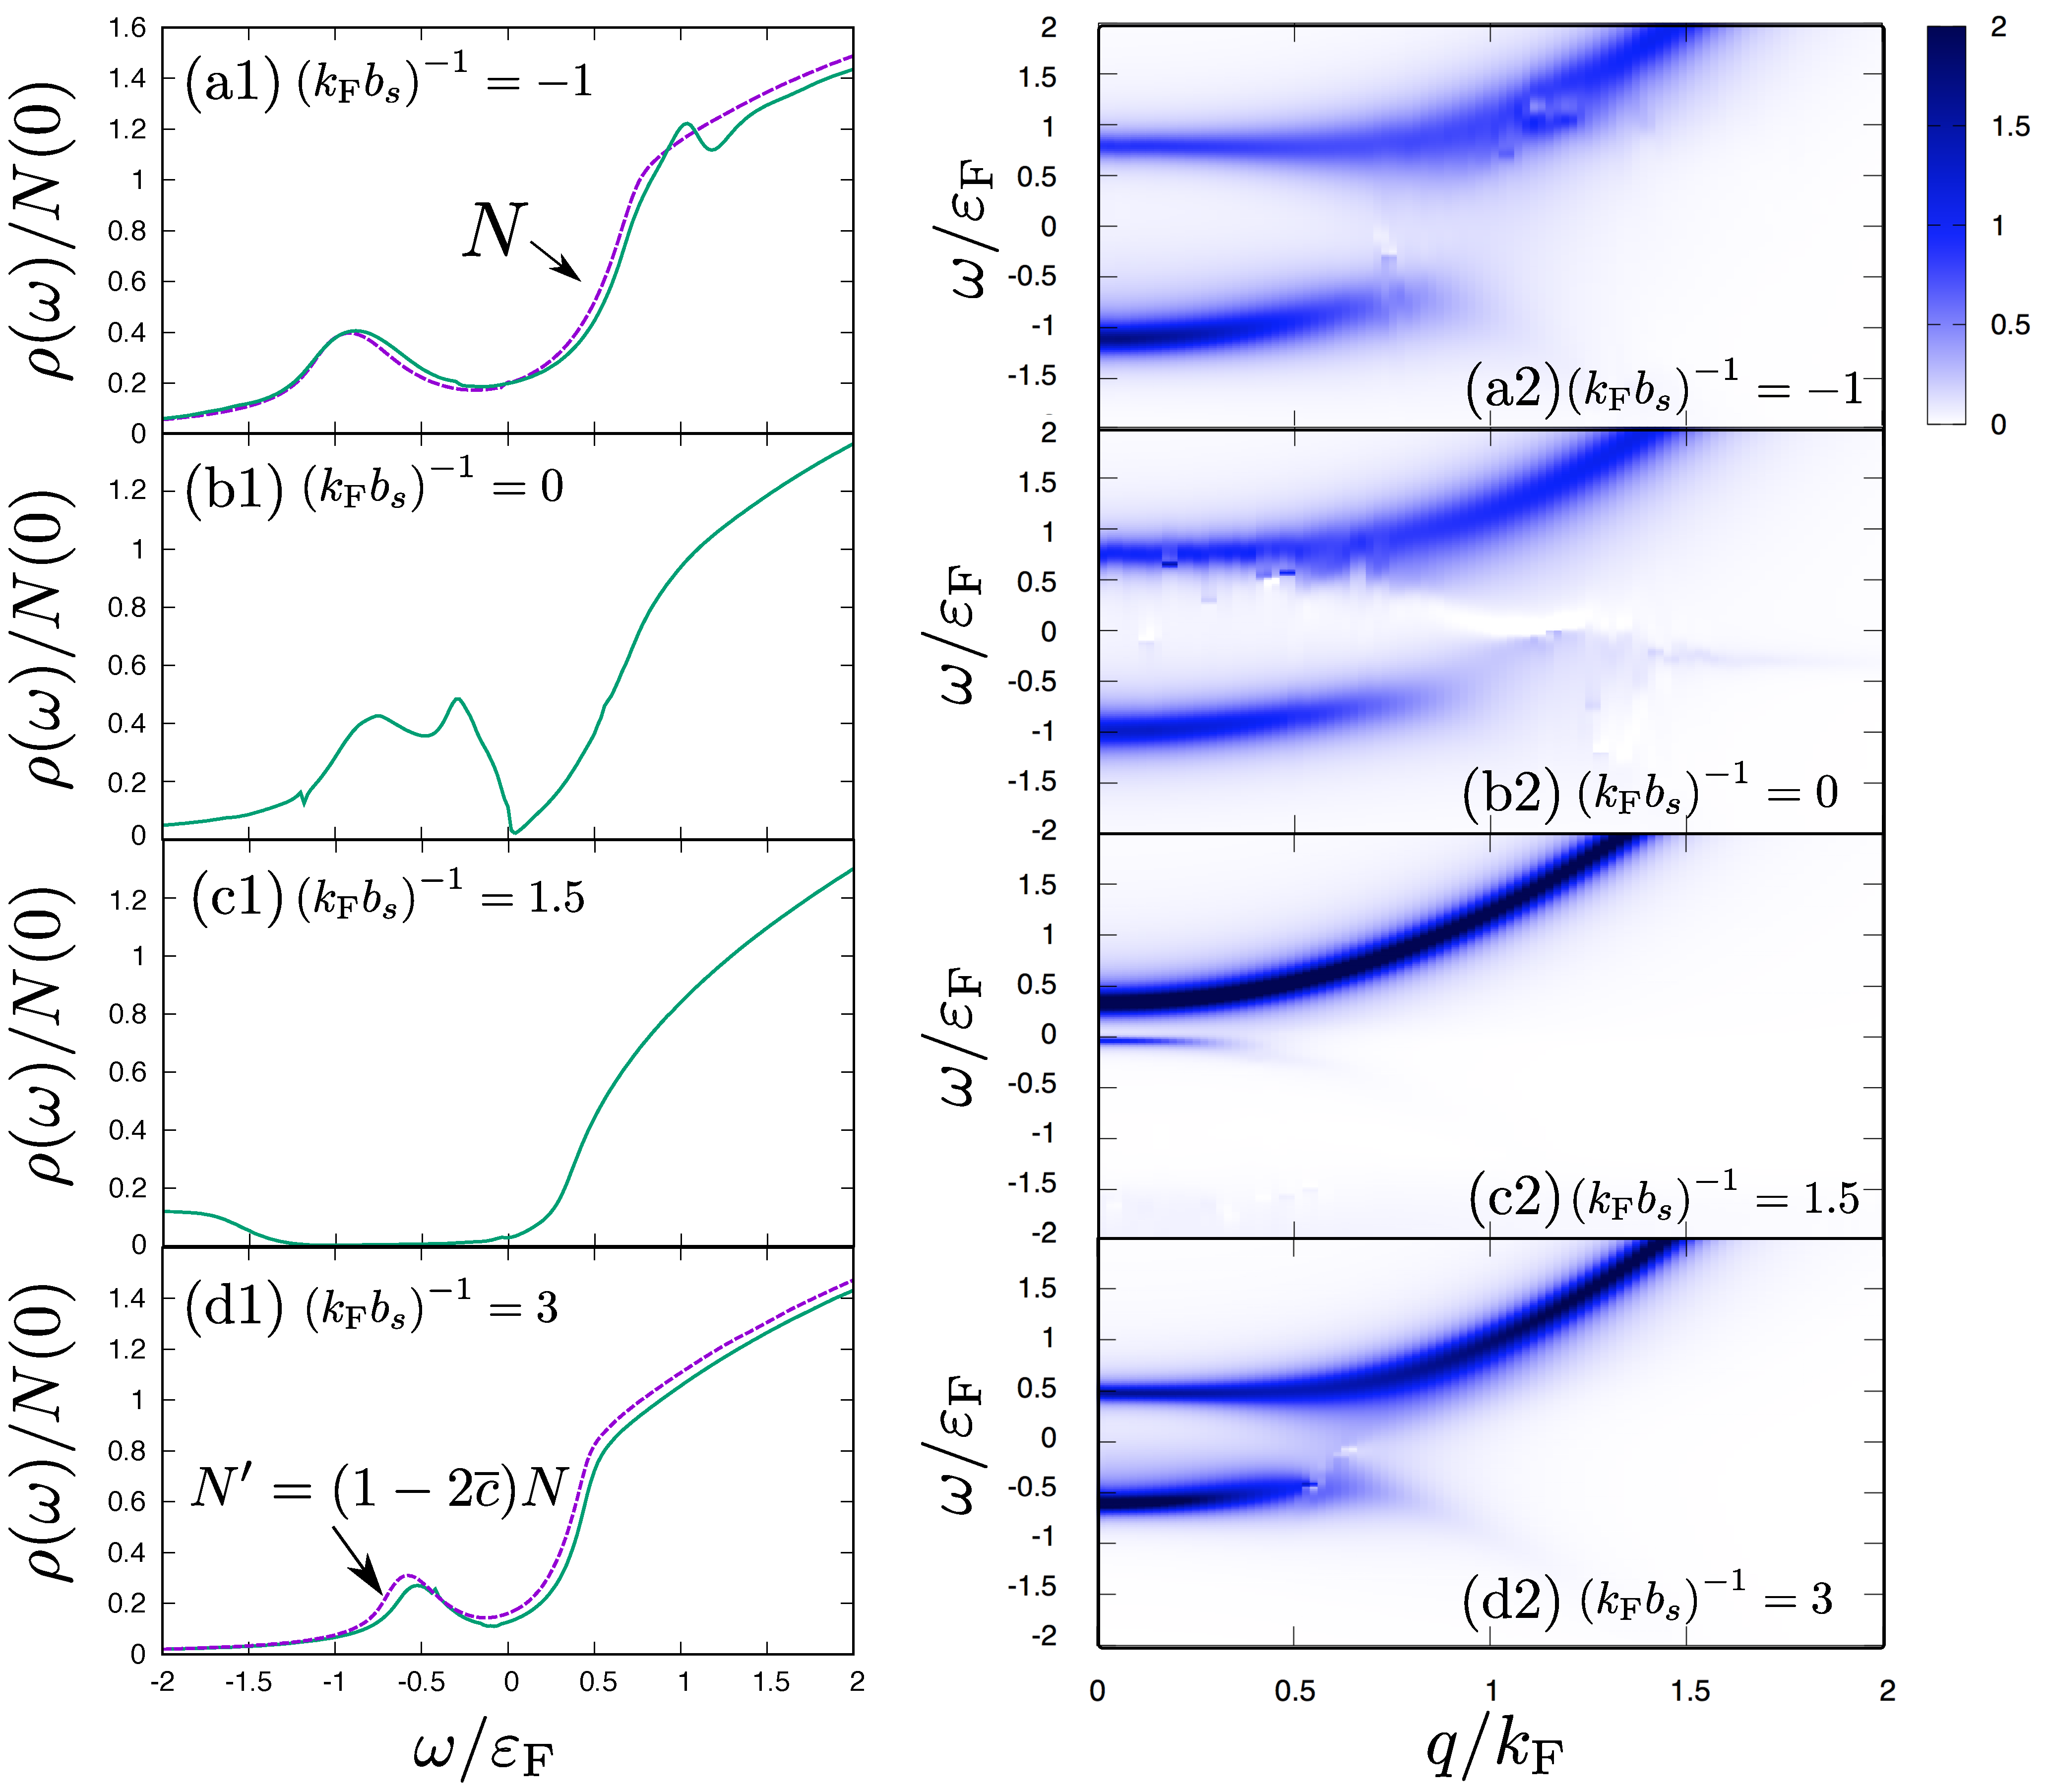
\includegraphics[width=130mm]{eps/tma-c0250-spe.eps}
\caption{$\overline{c}=0.25$、$T=\tc$ における 1 粒子状態密度(左)とスペクトル強度(右)。原子間引力相互作用はユニタリ極限 $\askfi=0$ にとってある。(a1) の破線は $N$ 粒子のクリーン系、(d1) の破線は $N'=(1-2\lc)N$ 粒子のクリーン系における擬ギャップ構造を有する状態密度。}
\label{fig:bcsl:imp:psgap}
\end{figure}

\begin{figure}[t]
\centering
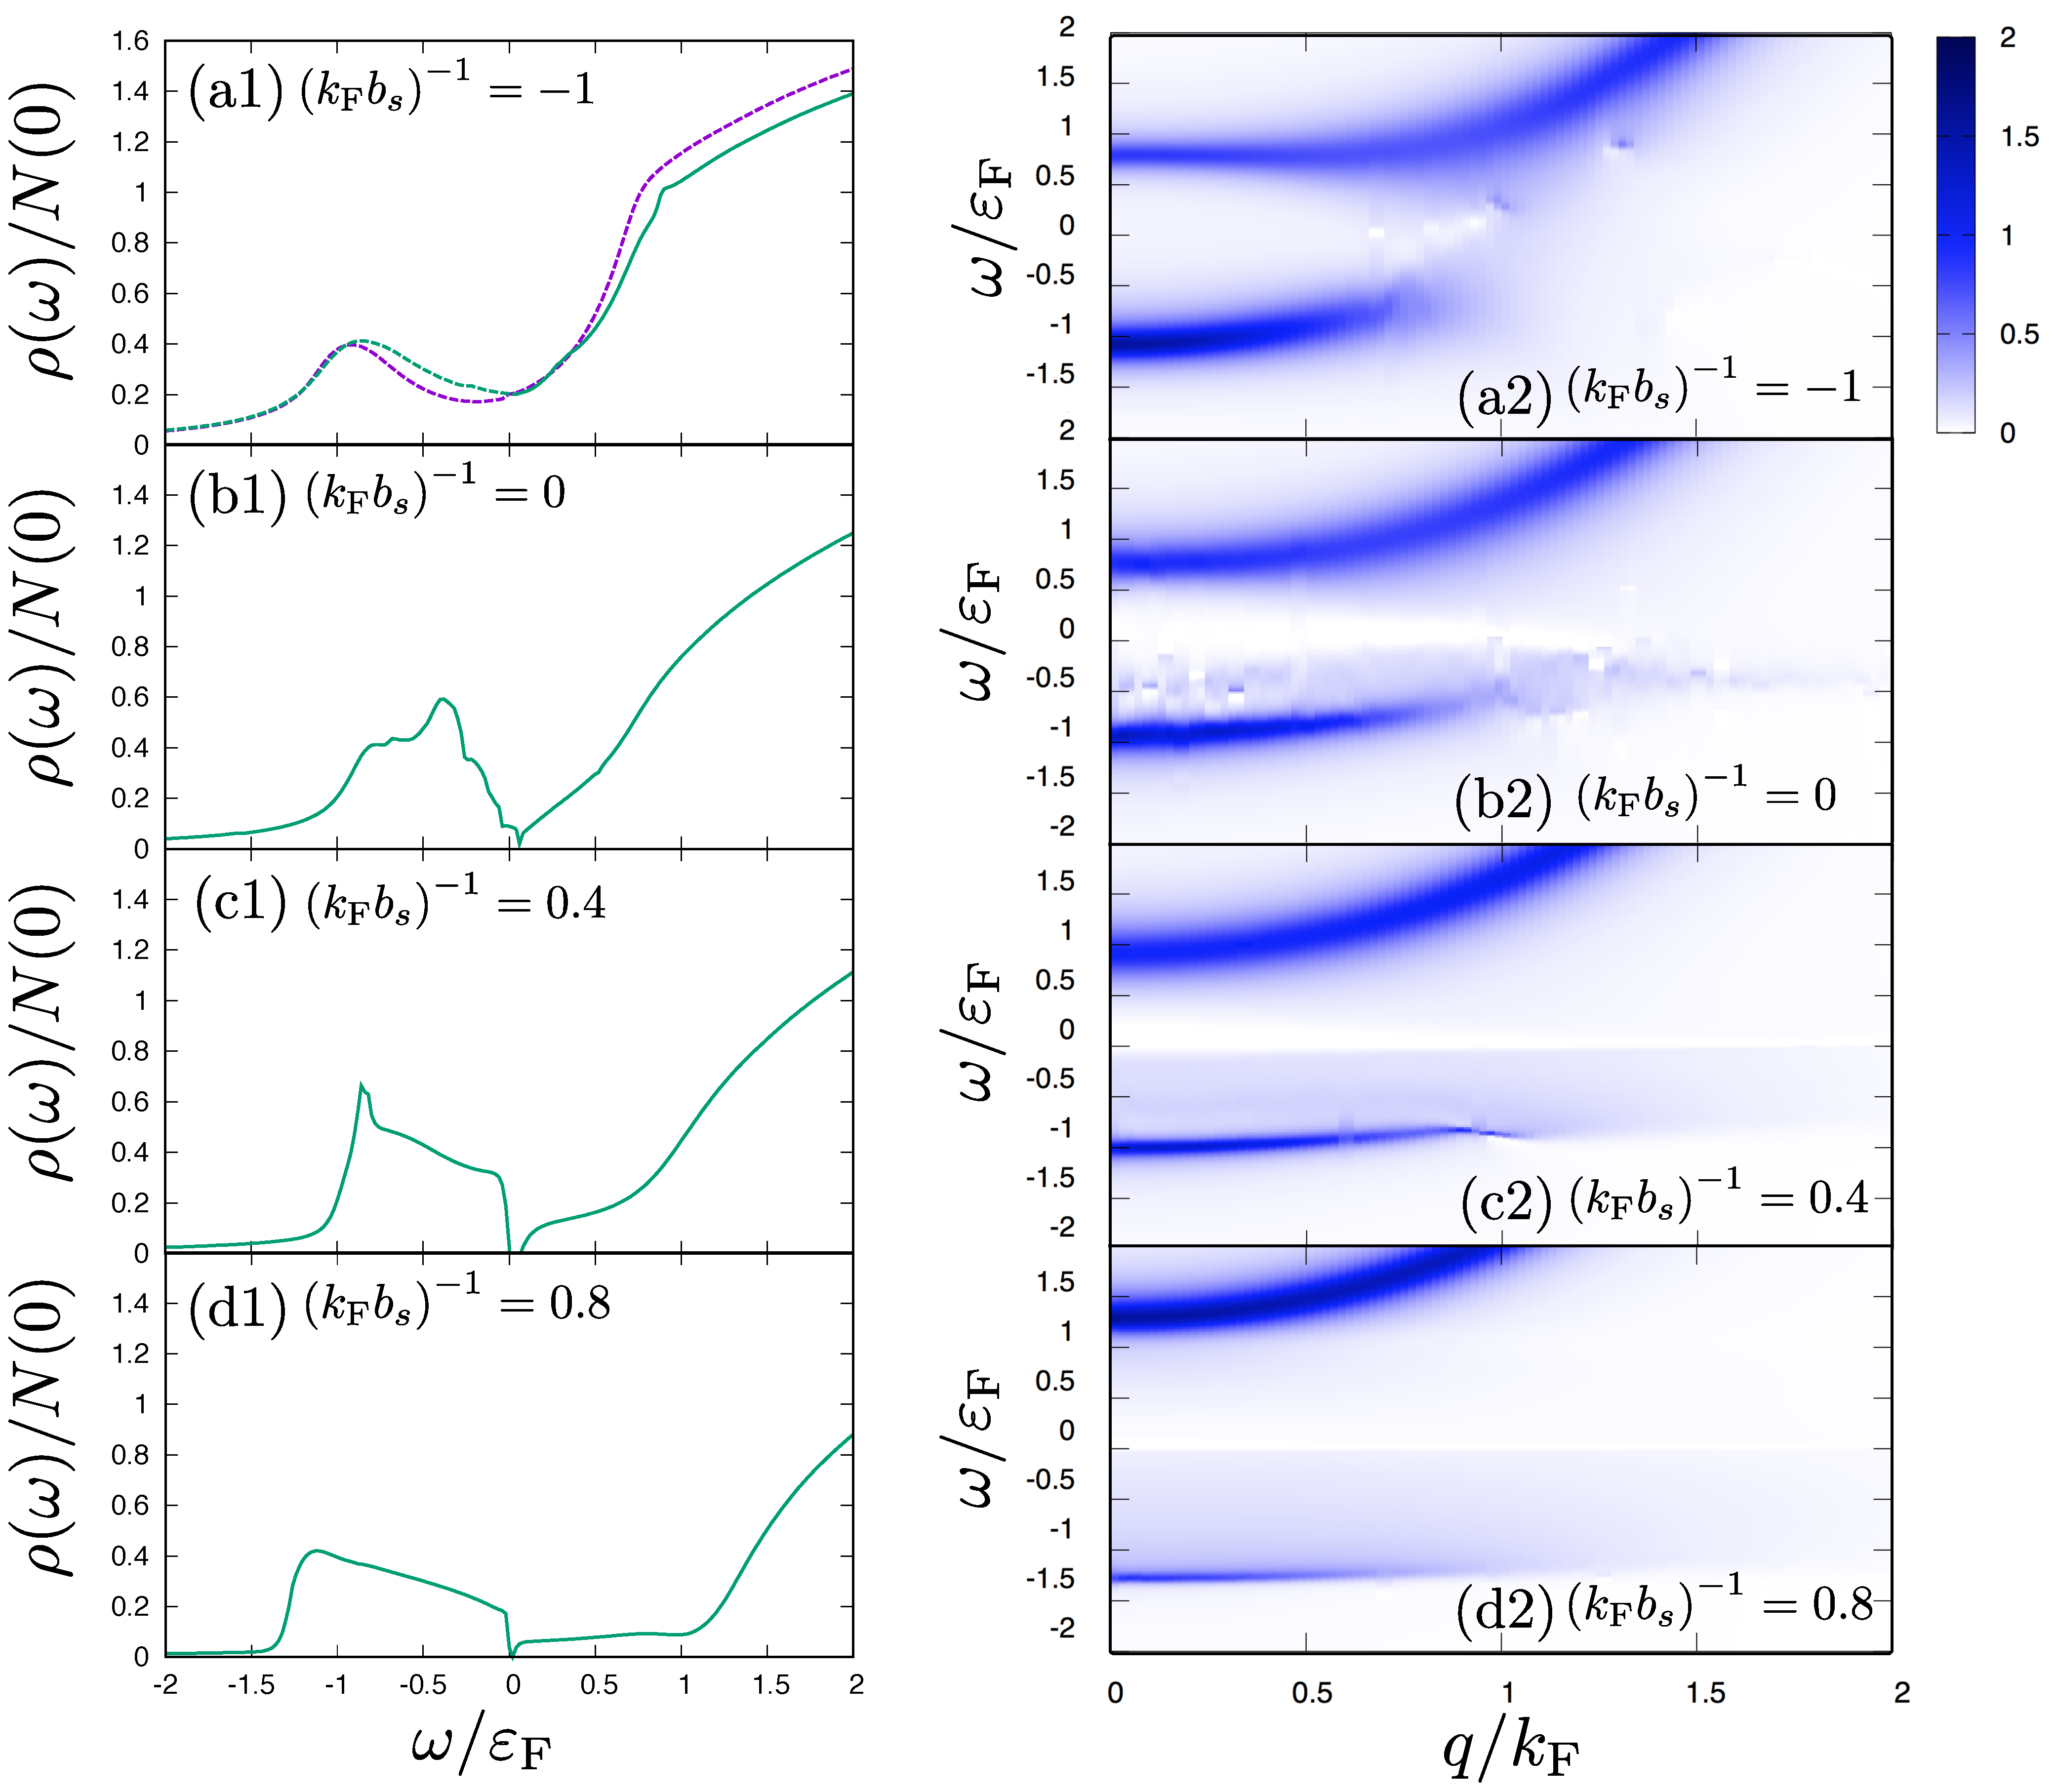
\includegraphics[width=130mm]{eps/tma-c0500-spe.eps}
\caption{図 \ref{fig:bcsl:imp:psgap} と同じだが $\overline{c}=0.5$ の場合。}
\label{fig:bcsl:imp:psgap1}
\end{figure}

\begin{figure}[t]
\centering
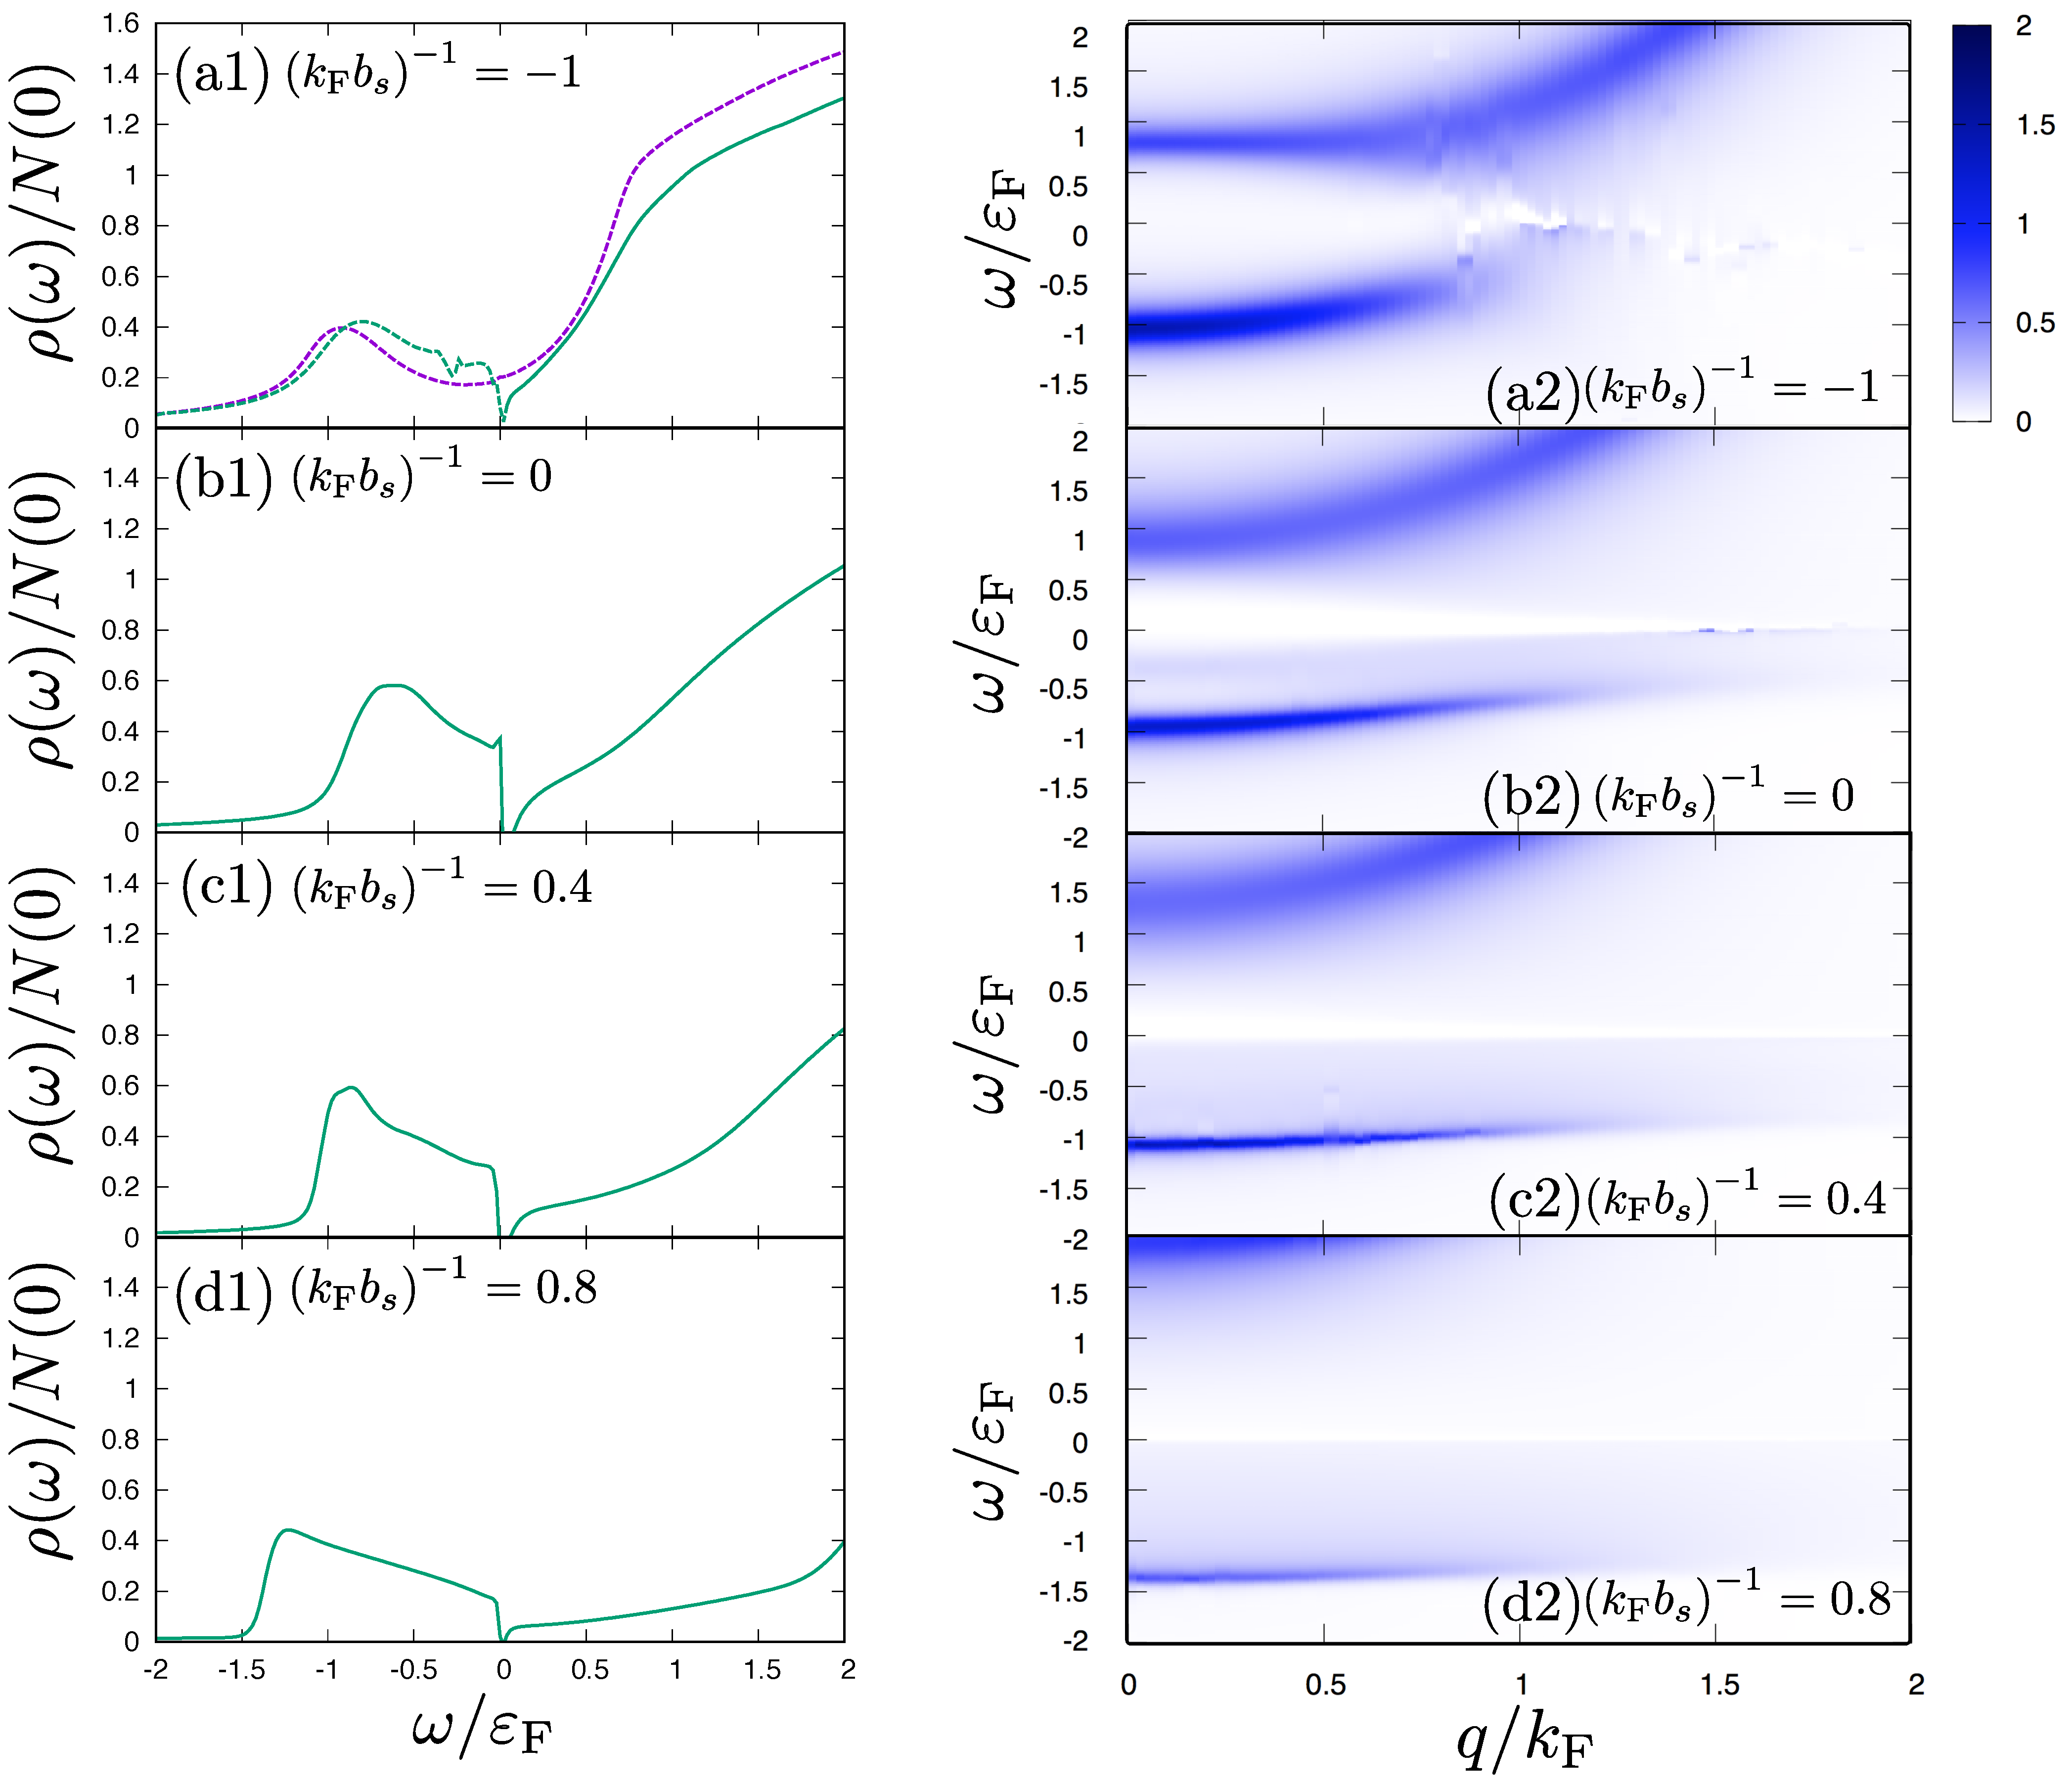
\includegraphics[width=130mm]{eps/tma-c1000-spe.eps}
\caption{図 \ref{fig:bcsl:imp:psgap} と同じだが $\overline{c}=1$ の場合。}
\label{fig:bcsl:imp:psgap2}
\end{figure}


式 (\ref{eq:bcsl:con:tctc0}), (\ref{eq:bcsl:con:cpcp0}) に見られるような $N'=(1-2\lc)N$ 粒子系への移行は擬ギャップ現象にも見られる。
擬ギャップ現象とは、超流動ゆらぎによって非凝縮のクーパー対が形成されることで、超流動転移温度以上においても超流動ギャップと同様に 1 粒子状態密度のフェルミ面近傍に窪み構造が現れる現象である。図 \ref{fig:bcsl:imp:psgap} に示すように不純物散乱強度が弱い場合のユニタリ極限の 1 粒子状態密度には擬ギャップが見られるが、これは、不純物がない場合の擬ギャップ構造とほとんど同じである(不純物がない場合の結果と完全に一致しないのは、図 \ref{fig:bcsl:imp:ndosc0500} の常流動状態における状態密度から、$\bskfi=-1$ の段階で自由粒子の底が $\omega+\mu=0$ から立ち上がらなくなっていることから、すでに多少の不純物準位の影響を受けているためであると考えられる)。ここから不純物散乱強度を強くしていくと、最終的には $N'=(1-2\lc)N$ 粒子系のユニタリ極限における(擬ギャップ構造のある) 1 粒子状態密度に帰着することがわかる。図 \ref{fig:bcsl:imp:psgap} の右側に示すように、スペクトル強度 $A_{\bp}(\omega)$ も (a)$\to$ (d) を見ると、$N$ 粒子系の擬ギャップ構造から、$N'=(1-2\lc)N<N $ 粒子系の擬ギャップ構造に漸近する様子が見て取れる。

これに対し、$\bskfi\gg1$ で、全原子が不純物に束縛されてしまう $\lc=0.5$ の場合は、図 \ref{fig:bcsl:imp:psgap1} に示すように不純物散乱の効果が強くなるにつれ、擬ギャップ構造は消失するが、(d1) の状態密度は単純な不純物を有する自由フェルミ気体の状態密度とは異なっており、状態密度の詳細な構造には、超流動揺らぎの影響があることがわかる。これは $\lc=1$ の場合にも見られる効果である(図 \ref{fig:bcsl:imp:psgap2})。ただし、これら後者 2 つの場合、$\bskfi=0.8$ での状態密度の構造の詳細が超流動揺らぎのどういう性質を反映したものであるか、については今後の研究課題である。



